\documentclass[12pt,letterpaper]{article}
\usepackage[utf8]{inputenc}
\usepackage[english]{babel}
\usepackage{fancyvrb} %font size definition within verbatim
\usepackage{array}
\usepackage{amsmath}
\usepackage{amsfonts}
\usepackage{amssymb}
\usepackage{amsthm}
\usepackage{graphicx}
\usepackage[left=2cm,right=2cm,top=2cm,bottom=2cm]{geometry}
\usepackage{array}
\usepackage{calc}
\usepackage{fancyhdr,graphicx}
\usepackage{setspace}
\usepackage{tabularx}
\usepackage{booktabs}
\usepackage[bottom]{footmisc}%pied de page à la fin 
\usepackage{authblk}
\usepackage{multirow}
\usepackage{xcolor}
\definecolor{mygreen}{rgb}{0.13, 0.55, 0.13} %forrest green

\newcolumntype{Y}{>{\raggedleft\arraybackslash}X}% raggedleft column X
\newcolumntype{C}{>{\centering\arraybackslash}m{2cm}}
\usepackage{makeidx}
\usepackage[separate-uncertainty = true,multi-part-units=single]{siunitx} 
\usepackage{caption}
%\usepackage{paralist}
%\usepackage{tablefootnote}
\usepackage{pdflscape}% necessary for landscape
\usepackage{afterpage}% necessary for landscape
\usepackage{capt-of}% necessary for landscape.or use the larger `caption` package
\usepackage{adjustbox}
\usepackage{apalike}
\usepackage{hyperref}
\usepackage{nameref} %title as name references not only section number
\usepackage{float}
\usepackage[toc,page]{appendix}
\usepackage{placeins} 
\usepackage{textgreek}
\usepackage{epigraph}
\usepackage{multicol}

\usepackage{ragged2e }
\setlength{\epigraphwidth}{0.8\textwidth}

%\noindent\hrulefill %graphicx package
%\smallskip\noindent %graphicx package

\doublespacing

%Biblio

\usepackage[apaciteclassic]{apacite}
%\usepackage[backend=bibtex,style=numeric-comp ,natbib=true]{biblatex}
%\addbibresource{BridgeBib.bib}
\bibliographystyle{apacite}

\begin{document}


%
%\title{Good Portfolio Management without Reinventing the Wheel}
\title{Good Portfolio Mgmt. without Reinventing the Wheel \footnote{
skyler.schneekloth@gmail.com;
I thank faculty director John H. Lewis for his contributions \& research guidance.}}


\author{Skyler Schneekloth}
\affil {University of Iowa \\ Tippie College of Business}



\maketitle              % typeset the header of the contribution
%

\begin{abstract}
%The Efficient Market Hypothesis (EMH) is a cornerstone of financial economics deeply entrenched in business school curricula, influencing a trend towards passive investing throughout the 21$^{st}$ Century. Proponents of EMH believe it's impossible to \textit{consistently} beat the market over an extended period due to the rapid assimilation of information into stock prices. Yet the notable long-term successes of investors such as Warren Buffett and top-performing hedge funds like Millennium Global clearly challenge this premise. This paper adopts a contrarian stance by evaluating various optimization algorithms used in active fund management, namely Markowitz-style strategies that have increasingly outperformed the S\&P 500 in CRSP data over the past decade. Our findings indicate that superior portfolio construction and monthly rebalancing is crucial for outperformance despite the challenges of linear transaction costs and significant estimation error in expected returns. Our results not only question the universal applicability of EMH over recent history, but also suggests how investors might skillfully navigate financial markets moving forward without reinventing the wheel.


The Efficient Market Hypothesis (EMH) is a cornerstone of financial economics and influences the trend towards passive investing. Yet, consistent outperformance by investors like Warren Buffett and certain hedge funds challenge this premise. Our paper implements R-based optimization algorithms that have increasingly outperformed the S\&P 500 in CRSP data over the last decade. Our findings emphasize the importance of effective portfolio construction in achieving abnormal returns, despite linear transaction costs and estimation errors. Results challenge the universal applicability of EMH and propose ways for investors to skillfully navigate financial markets without reinventing the wheel.

\end{abstract}

{\Centering
Presented to the Faculty of the Graduate School of the University of Iowa in partial fulfillment of the requirements for the degree of Master of Science in Finance \par}

\vspace{0.5cm}

{\Centering
Data Repository: \href{https://github.com/SkylerSchneekloth/Thesis-in-Portfolio-Optimization}{https://github.com/SkylerSchneekloth/Thesis-in-Portfolio-Optimization}}

\newpage

\section{Introduction}

According to \citeA{SPDowJones2023}, “approximately 25\% to 33\% of the S\&P 500 was held within passive portfolios by 2021” representing a steep increase in the overall quantity of passively managed AUM since 2010. \$10.1 trillion---nearly one-third of the \$33.6 trillion U.S. retirement market---is currently invested in mutual funds and, according to the \textit{2023 Investment Company Fact Book} published by the Investment Company Institute (ICI), “index mutual funds’ share of long-term mutual fund net assets [including DC plans and IRA assets] more than tripled, from 7.5 percent at year-end 2000 to 27.9 percent at year-end 2022". Furthermore, “within index mutual funds, index equity mutual funds accounted for the bulk (81 percent) of index mutual fund total net assets at year-end 2022” according to the ICI report. Overall, 62\% of all IRAs and 401(k) plans are equity investments, increasingly passively managed \cite{ICI2023Factbook}. With so many Americans depending on the stock market for a prosperous retirement, wealth managers have a fiduciary responsibility to identify and utilize the most effective asset allocation models. Is the trend towards passive management justified within this context? In this paper, we put several optimization algorithms to the test, pitting them against the S\&P 500 over a 29-year period.

Modern Portfolio Theory (MPT) has come a long way since Harry Markowitz. Researchers have undeniably introduced superior versions of mean-variance optimization (MVO) by publishing articles over the past few decades. These newer, better models are less sensitive to estimation error and have good mechanisms for handling uncertainty. Does that mean long-term investors should throw MVO out the window? While acknowledging significant contributions to MPT since Markowitz, we argue that MVO is still a reliable algorithm for weighting large-cap stocks in the United States between 2010 and 2023, even when expected returns are not perfectly estimated.

The next section is a brief literature review highlighting two extensions of MVO that control for uncertainty in parameter estimates---shrinkage and Resampled Efficiency. In section 3 we discuss our dataset, explain our methodology for removing bias from backtests, and interpret results. The final section is split between our suggestions for future research and a conclusion. Empirical evidence indicates that several actively-managed portfolios have consistently outperformed the S\&P 500 over an extended period despite linear transaction costs and estimation error.

\section{Literature Review}

According to \citeA{handa06}, “it is worth asking whether belief in predictability of returns translates into economically significant gains that are sustainable”. The authors examine the potential for stock return forecasts to enhance asset allocation strategies and investment performance in the U.S. stock market from 1954 to 2002, using various statistical methods to examine how predictability might shape the efficient frontier. Their findings suggest that incorporating return predictability into asset allocation models does not guarantee superior long-term performance---“our results serve to underscore the fact that translating the predictability that exists in data into consistently superior performance is challenging, and therefore investment strategies that rely on data-based predictor variables should be tempered with caution” \cite{handa06}. This suggests that sophisticated forecasts of asset-level returns do not always translate into better portfolio performance, and estimation error might not be as critical an issue as previously assumed. Therefore, it may be more productive to concentrate on portfolio construction rather than forecasting expected returns.

Let us start with Harry Markowitz, who solidified his reputation as the godfather of MPT after winning the 1990 Nobel Price in Economics for inventing mean-variance portfolio optimization (MVO) nearly 75 years ago \cite{markowitz52}. By consensus opinion, “Markowitz had the brilliant insight that, while diversification would reduce risk, it would not generally eliminate it” \cite{rubinstein02}. Fund managers have aimed to maximize Sharpe Ratios ever since, and refined versions of MVO have emerged from scholarly research. The article “Portfolio Selection” \cite{markowitz52} is truly seminal.

Despite prevailing as the textbook example of portfolio optimization, MVO is chiefly scrutinized for being highly sensitive to estimation error in expected asset returns. Critics argue there is no way to reliably control for uncertainty within the Markowitz framework. Additionally, MVO unfortunately tends to overweight the riskiest assets to maximize its return objective hence failing to capture a diversification benefit, although this can usually be corrected by imposing a minimum and/or maximum allocation constraint on the stock pool. Recent literature has introduced more advanced approaches for addressing estimation error.

\citeA{ledoitwolf03} propose a regularization method that “shrinks” the variance-covariance matrix of risky asset returns toward the average of its off-diagonal elements. That is: a process that systematically adjusts extreme coefficients towards the first central moment, thus achieving more reasonable expectations for cross-asset variances (think of shrinkage intensity as a lasso that reigns in extreme outliers). This approach is statistically grounded, with a formula provided for optimal shrinkage intensity, and it is claimed to be superior to Markowitz optimization. Applied to actual stock market data, the shrinkage method reduces tracking error relative to a benchmark index and significantly increases the realized information ratio of active portfolio managers. Since 2003, others \cite{bodnar22, pedersen21} the have built on the Ledoit and Wolf model. For example, \citeA{pedersen21} introduces two versions of “Enhanced Portfolio Optimization” (EMO)—“simple” versus “anchored”—both developed to address estimation error with shrinkage. However, in contrast to \citeA{ledoitwolf03} and \citeA{bodnar22}, \citeA{pedersen21} utilizes a much higher shrinkage intensity to “fix” the covariance matrix. In this article, a shrinkage intensity of about 5\%-10\% suffices to correct errors in the risk model, but a much larger shrinkage intensity (about 75\%) is required to improve portfolio Sharpe Ratios. The main innovation of \citeA{pedersen21}  is the use of  Principal Components Analysis (PCA) to specifically identify “portfolios that cause problems in standard MVO”, enabling a more precise application of shrinkage to the variance-covariance matrix of risky asset returns than performed in \citeA{ledoitwolf03} and \citeA{bodnar22}.

\citeA{michaud07} develop an alternative to \citeA{ledoitwolf03} called Resampled Efficiency (RE). The RE method is a very intuitive way to address estimation error and poor out-of-sample performance. The article proposes a Monte Carlo with the number of simulations being set proportional to the portfolio manager’s certainty regarding his expected return estimates---the more confident in his calculations, the greater number of simulations the fund manager runs to model an efficient frontier. The RE method technically relies on bootstrap (i.e., sampling with replacement) from the normal distribution (or some other, known/assumed distribution) and theoretically depends on the Central Limit Theorem. Unfortunately, the RE methodology is patented and cannot be used in practice.

Given the advancements in addressing estimation error by \citeA{ledoitwolf03}, \citeA{bodnar22}, \citeA{pedersen21} and \citeA{michaud07}, it seems plausible that portfolio optimization has become more robust and hence capable of outperforming the market. Perhaps even when expected returns are poorly estimated.

\section{Backtesting Portfolios}

\subsection{Data Sources and Data Pre-Processing}
Our data was fetched from CRSP via Wharton Data Research Services (WRDS). Since S\&P Dow Jones Indices constituent name data was licensed and removed from Compustat in July 2020,\footnote{For more information, see \href{https://wrds-www.wharton.upenn.edu/pages/support/support-articles/compustat/north-america/compustat-index-constituents-removed/}{WRDS documentation on Compustat index constituents}.}
we purchased the complete constituent history from Siblis Research to manage survivorship bias. We compiled a unique ticker list from this data, which we used to access monthly stock files on CRSP from December 1989 to December 2023. This provided us with asset-level price returns (i.e., excluding dividends) and total returns (i.e., including dividends). Adjustments were necessary to align Siblis tickers with CRSP identifiers, but no other modifications were made to the CRSP output.


Our asset-level returns are the monthly Holding Period Returns (ret) from the CRSP Annual Update.\footnote{“Databases in this section are updated once each year, in early February. Update schedules should not be confused with end-of-day, end-of-month, or end-of-quarter data such as stock prices.”} We perform standard calculations on these returns throughout backtesting to derive variance-covariance matrices and the mean vector, serving as inputs for optimization.

Our risk-free rate is the 30-day TBill rate of return sourced from the U.S. Treasury and Inflation Indexes data series on CRSP. We use this rate to calculate portfolio-level Sharpe Ratios and Treynor Ratios, which measure risk-adjusted returns.

\subsection{Methodology}

\subsubsection{Calculating Expected Returns}
We calculate expected returns as 60-month arithmetic averages of the Holding Period Returns from CRSP, which is nothing fancy. Recall the purpose of this article: to demonstrate that mean-variance portfolio optimization can beat the market despite estimation error in expected returns. Our expected return estimates are not perfect, in fact they are very crude. This is intentional, and serves the purpose of underscoring the importance of optimization algorithms in portfolio design. We aim to prove that optimization is always worthwhile, even lacking asset return predictability.

In mathematical notation, the asset-level expected returns at $t_1$ are given by:
\begin{align}
E[R_{t_1}] = \sum_{i=t_0}^nR_i \text{ ÷ } n
\label{eq:expectedRetCalc}
\end{align}

where $R_i$ is the Holding Period Return in month $i$, $t_0$ is the starting period, and $n$=60 to capture 60 months of data between $t_0$ and $t_1$ (inclusive).

\subsubsection{Handling Time-Related Biases}
A proper backtest controls for look-ahead bias and survivorship bias. Look-ahead bias is an error that occurs when the researcher uses information that would not have been available at the time of the analysis, leading to inaccurate results. In financial modeling, look-ahead bias arises when a model incorporates data or events that have not yet occurred at the point in time being analyzed. Look-ahead bias skews the results of backtesting, often making investment strategies appear more profitable or less risky than they actually are. Survivorship bias is a form of selection bias occurring when an analysis focuses solely on entities which have “survived” the course of history. In financial modeling, survivorship bias typically refers to the misconception that the active constituents of a market index (such as the S\&P 500 constituent list, which is updated quarterly) have \textit{always} and exclusively prevailed as constituents. Like look-ahead bias, survivorship bias usually inflates the attractiveness of the investment strategies which are being tested.

\clearpage

To neutralize look-ahead bias, we first lag the ticker history by one period such that our stock universe is limited to companies listed on the S\&P 500 in that moment i.e., only tickers observed at the \textit{end of the prior month}. For example, we use the ticker list observable on 1994-12-31 to obtain weightings for the month of Jan 1995. According to Siblis Research, the S\&P 500 index constituents are updated each quarter until Jun 2016 and potentially change on a monthly basis thereafter. In our analysis, an active portfolio manager rebalances on the first of every month. So, asset-level returns are also lagged by exactly one period (since these, too, are reported at month-end). For example, the expected monthly return on stock XYZ in Dec 2023 is the 60-month arithmetic average of XYZ's return stream from Dec 2018 to Nov 2023, not Jan 2019 to Dec 2023 (since the month-end closing price in Dec 2023 is unknown on Dec 1, 2023). The portfolio's monthly return on 2023-12-31 is then calculated as a weighted average of asset weights (obtained by solving the MVO problem with lagged data) and their actual monthly returns from Dec 2023 (i.e., the original/unlagged returns). By this process, which is designed to capture the monthly performances a fund manager would observe in real time, our portfolio-level returns are evaluated on a rolling out-of-sample basis. We call it “portfolio optimization with imperfect information”.

Our portfolio-level analysis spans from January 1, 1995, to December 31, 2023, covering a 29-year historical period (348 months). This timeframe accounts for a one-month lag to control for look-ahead bias and the need for 60 months of data to calculate expected returns, given that our asset-level CRSP data begins on December 31, 1989.

\subsubsection{Calculating Optimal Asset Weights}
\textcolor{blue}{PortfolioBacktester.R} utilizes the \textcolor{blue}{glpk} solver and several R packages to perform optimization within a \textit{for loop}. Each iteration of the loop submits expected returns and a covariance matrix to a quadratic optimizer, which then computes the optimal weighting scheme for its objective function. For example, we leverage the \textcolor{blue}{PortfolioAnalytics} and \textcolor{blue}{ROI} libraries to obtain our MVO portfolios which maximize portfolio-level return subject to 1) a full investment constraint and 2) user-defined minimum/maximum asset-level allocation constraints. The RE portfolios also use \textcolor{blue}{PortfolioAnalytics} and \textcolor{blue}{ROI}, except the optimal weights are averages of a Monte Carlo process that samples a mean vector and covariance matrix of returns from a normal distribution centered at the original (point estimate) values normally used in MVO until enough observations are available for convergence, as instructed by \citeA{michaud07}. In \citeA{michaud07}, the number of simulations is set proportional to the investor's confidence in his expected return estimates. We test both 50 and 100 simulations and subject the RE optimizer to a 2.5\% maximum allocation constraint in Table \ref{tab:performance_metrics_table}. All our MVO and RE portfolios are long-only.

We use \textcolor{blue}{HDsHOP} to apply the optimal covariance penalty as suggested by \citeA{ledoitwolf2020}. The adjusted “shrunk” covariance matrix is then passed to the \textcolor{blue}{portfolio.optim()} function from \textcolor{blue}{tseries}---a quadratic optimizer that enforces the user-defined minimum/maximum asset-level allocation constraints. Unlike \textcolor{blue}{PortfolioAnalytics} and \textcolor{blue}{ROI}, we can permit shorts within \textcolor{blue}{tseries}. This process gives us our Ledoit-Wolf portfolio, which is a long-short portfolio.

We use \textcolor{blue}{HDsHOP} exclusively for Bodnar-style shrinkage. Like the Ledoit-Wolf portfolio, the Bodnar portfolios are long-short. Unlike the Ledoit-Wolf, MVO, and RE portfolios, the Bodnar portfolios are not subject to any kind of minimum or maximum asset-level allocation constraint (they are only subject to a full investment constraint).

\subsubsection{Calculating Portfolio-Level Risk and Return Metrics}
\textcolor{blue}{PortfolioBacktester.R} outputs a single-column vector of portfolio-level returns, which are the weighted averages of lagged monthly asset returns and the optimal weighting scheme across ticker symbols. This gives us the portfolios out-of-sample performance for each month between 1995 and 2023. Form here, we calculate the following portfolio-level metrics presented in Table \ref{tab:performance_metrics_table}:

\begin{multicols}{2}    % Start a two-column environment
\begin{itemize}
\singlespacing
    \item Sharpe Ratio
    \item Treynor Ratio
    \item 3y monthly Beta, $\beta$
    \item Volatility (Standard Deviation)
    \item Historical 5\% VaR
    \item Historical 5\% CVaR
    \item Maximum Drawdown
    \item Minimum monthly return
    \item Maximum monthly return
    \item Compound Annual Growth Rate (CAGR)
    \item Average Monthly Portfolio Turnover
    \item Terminal Wealth
\end{itemize}
\end{multicols}

The Sharpe Ratios and Treynor Ratios follow the 2011 CFA GIPS standards \cite{cfaStandards} and the denominator for Treynor is the asset's 3y monthly Beta, which equals the slope of a simple linear regression of the S\&P 500's monthly Holding Period Return on the asset's monthly Holding Period Returns. Volatility is calculated as the standard deviation of monthly portfolio-level returns. 5\% VaR is the fifth percentile of historical monthly portfolio-level returns and 5\% CVaR is the corresponding expected shortfall based on the historical distribution. Maximum Drawdown is based on a \$1000 wealth index, but expressed in percentage terms. Minimum and maximum monthly returns are the lowest and highest between January 1995 and December 2023, respectively. CAGR is a geometric average over the same period. Terminal wealth is the closing balance from a \$1000 investment submitted to each portfolio at the beginning of 1995, at the end of 2023---it is the final observation in Figure \ref{fig:TotRetWeatlhIndexWithTransactionCosts} (panel A) and Figure \ref{fig:TotRetWeatlhIndexWithoutTranactionCosts} (panel B). We separate calculations with transactions (panel A) from calculations without transaction costs (panel B); transaction costs are calculated in the next sub-section alongside turnover. All calculations were performed in RStudio 2023.12.1+402 and double-checked in Microsoft Excel for arithmetic. Files are available for download at the GitHub link.

\subsubsection{Calculating Turnover and Transaction Costs}
We adopt \citeA{handa06}'s 50 basis points round-trip assumption and therefore multiply portfolio turnover by 0.0025 to compute monthly transaction costs from January 1995 to December 2023. Turnover is defined as the percentage of the portfolio's composition that changes MoM. It is calculated as the sum of the absolute differences between the weights of the portfolio at the beginning and the end of each month, divided by two. The division by 2 adjusts for how turnover is accounted for in buying and selling transactions. When selling one security and buying another, the total portfolio change includes both the sale and the purchase, but the actual “new” money involved is only on one side of these transactions. Turnover results from monthly portfolio rebalancing. For simplicity, we assume that transaction costs are linearly proportional to portfolio turnover (although research shows that transaction costs are in fact nonlinear).

\clearpage

In mathematical notation, turnover in month $t$ is calculated over a portfolios holdings $i$ as the sum of their absolute differences divided by 2:
\begin{align}
(\sum_{i} | w_i^{t} - w_i^{t-1} |) \text{ ÷ } 2
\label{eq:turnoverCalc}
\end{align}

and transaction costs given by:
\begin{align}
[(\sum_{i} | w_i^{t} - w_i^{t-1} |) \text{ ÷ } 2]*0.0025
\label{eq:costsCalc}
\end{align}

where 0.0025 is a 25 basis point transaction charge that is linearly proportional to portfolio turnover. Therefore, transaction costs are highest for portfolios with a large average monthly turnover rate. Equation \ref{eq:costsCalc} is subtracted from monthly portfolio-level returns to adjust them for transaction costs before calculating the metrics presented in Table \ref{tab:performance_metrics_table} panel A.

\subsection{Results}

If you put \$1000 in the S\&P 500 on January 1, 1995 and held it until January 1, 2024 you would have \$17.9 thousand in the bank (ignoring taxes). By contrast, a \$1000 investment in MVO returned \$24.4 thousand over the same period representing a 36\% upside over passive investing despite linear transaction costs and estimation error in expected returns. This disparity has become more pronounced over the past decade according to Figure \ref{fig:TotRetWeatlhIndexWithoutTranactionCosts} and Figure \ref{fig:TotRetWeatlhIndexWithTransactionCosts}, the gap between MVO and the S\&P widening over a 10-year period between 2013 and 2023. The same trend is observed in Figure \ref{fig:TotRetWeatlhIndexWithoutTranactionCosts} for sophisticated optimization strategies such as shrinkage and Resampled Efficiency. However, after accounting for transaction costs in Figure \ref{fig:TotRetWeatlhIndexWithTransactionCosts}, the Bodnar portfolio's performance re-aligns with benchmark-level wealth generation between March 2021 and December 2023; this adjustment is due to extremely high monthly turnover in the Bodnar portfolios as show in Table \ref{tab:performance_metrics_table}. Therefore, the Bodnar portfolios may stand to benefit from a monthly turnover constraint.\footnote{Note that the current version of \textcolor{blue}{HDsHOP} does not accommodate turnover constraints.}

Turning attention to panel A of Table \ref{tab:performance_metrics_table}, which considers transaction costs, nearly half of the alternate portfolios generated more wealth than the S\&P 500 out-of-sample---MVO with a 2.5\% maximum asset allcoation constraint, the Bodnar shrinkage portfolio with its risk parameter set equal to $\gamma=250$, and both Resampled Efficiency (RE) portfolios. The Bodnar portfolio with its risk parameter set equal to $\gamma={50,100}$ generated comparable wealth to the benchmark but did so with more return per unit of total risk---1\% and 0.9\% higher monthly Sharpe Ratios than the S\&P 500, respectively. The Ledoit-Wolf portfolio underperformed the S\&P 500 after accounting for transaction costs.

Shrinkage portfolios do a much better job at managing risk than MVO and RE by all measures (volatility, VaR, CVaR, and Max Drawdown), both with and without transaction costs. For example, investors in the Ledoit-Wolf portfolio face a 5\% probability of losing more than 5.8\% in any given month between January 1995 and December 2023 and can expect to lose 8.4\% when returns drop below the fifth percentile of the portfolio's historical distribution. Investors in the Bodnar portfolios face a similar downside risk, but MVO and RE investors face larger 5\% historical VaR's and CVaR's. A passive investor splits the difference, facing a 5\% chance that the S\&P 500 will drop below 7.4\% in one month and lose 9.6\% beyond that point based on it's historical distribution of returns. According to Figure \ref{fig:drawdowns}, investors may be in for a bumpier ride going with MVO or RE versus Ledoit-Wolf or Bodnar. While MVO and RE portfolios experience deep drawdowns in bear markets because of their high Betas ($\beta>1$), the shrinkage methods take mild dips less drastic than the market itself. However, risk tolerant investors may be rewarded with a higher terminal wealth according to Table \ref{tab:performance_metrics_table}.

Shrinkage portfolios generally have the best out-of-sample Sharpe Ratios and Treynor Ratios on average from January 1995 and December 2023 and less exposure to market risk over the past three years. Shrinkage portfolios are the only actively-managed strategies that outperform the market in terms of risk-adjusted return, but fall short of MVO and RE in terms of wealth generation after transaction costs. By contrast, MVO and RE generate the greatest wealth \textit{despite} transaction costs, but take on more risk per unit of return than the S\&P 500. All of the actively-managed portfolios suffer from a high degree of estimation error in monthly rebalancing; yet 6 of 9 still manage to beat the market either with respect to wealth generation, risk-adjusted return, or both. These tend to be the more sophisticated version of MVO, but plain vanilla MVO with a 2.5\% maximum allocation constraint is also among our top-performers.

\subsubsection{High Turnover in Shrinkage Portfolios}

Observing the Bodnar and LW portfolios in panel A (includes transaction costs) and panel B (ignores transaction costs), we discover high average monthly turnover in all shrinkage-based optimization which negatively impacts performance. This suggests each of these portfolios stand to benefit from a monthly turnover constraint. Future research might explore the effects of such constraints or test alternative implementation in a different R package. \textcolor{blue}{HDsHOP}'s optimizer yields turnover close to randomization in our results, which is impractical.

Figure \ref{fig:gamma_vs_Twealth} demonstrates an obvious relationship between an investor's risk adversity ($\gamma$) and their terminal wealth on December 31, 2023. It suggests the optimal gamma value which maximizes terminal wealth, $\gamma^{*}$, might be somewhere between 25 and 60, given the horizontal asymptote of \$25,000 as $\gamma$ approaches 100. Our analysis in \textcolor{blue}{HDsHOP} required a much larger gamma value of $\gamma=250$ to really beat the market, which seems \textit{too} high. Again, future research might reconstruct the Bodnar portfolios and fine-tune the $\gamma$ hyperparameter outside of \textcolor{blue}{HDsHOP}.

\subsubsection{Markowitz vs. Resampled Efficiency}

In comparing MVO to RE, decreasing the maximum asset allocation constraint on MVO as shown in Figure \ref{fig:MarkowitzFrontiers} achieves similar efficient frontiers as decreasing the number of simulations in RE as shown in Figure \ref{fig:MichaudFigure5}, which means we can use max constraints to control for uncertainty in our expected return calculations within the MVO framework much like we would adjust the number of simulations in RE to reflect confidence in these parameter estimates. In other word, both portfolios have reliable mechanisms for handling estimation error.

Maximum allocation constraints ensure a predictable degree of diversification in MVO portfolios, always spread evenly across the optimal set of assets as depicted in Figure \ref{fig:MarkowitzCompositionMap}. Our composition maps for both MVO (Figure \ref{fig:MarkowitzCompositionMap}) and RE (Figure \ref{fig:MichaudCompositionMap}) are consistent with \citeA{michaud07}. Like \citeA{michaud07}, we observe a “smooth transition” across buckets in Figure \ref{fig:MichaudCompositionMap} compared to Figure \ref{fig:MarkowitzCompositionMap}. Here, the RE portfolio maintains its diversification under a maximum 50\% constraint, unlike the MVO portfolio. Hence, RE achieves superior diversification quality compared to MVO. Moreover, as Figure \ref{fig:MichaudCompositionMap} illustrates, RE could potentially benefit from a \textit{minimum} allocation constraint, as it encompasses a much broader range of stocks and exercises self-control in allocating dollars to the riskiest outliers. We find that RE also achieves a better diversification of factor exposure than MVO by comparing the correlation networks in Figure \ref{fig:MarkowitzCorrelationNetwork} versus Figure \ref{fig:MichaudCorrelationNetwork}. Nonetheless, both strategies yield similar risk-adjusted returns according to Table \ref{tab:performance_metrics_table}.

In this section, we compared the performance of different investment strategies from 1995 to 2024. Investing \$1,000 in the S\&P 500 on January 1, 1995 resulted in a terminal wealth of \$17,892 on December 31, 2023. The same initial investment in the MVO portfolio generated \$24,403 over the same 29-year period. The superior performance of MVO persists even after accounting for linear transaction costs and despite high estimation error in expected returns. Notably, a performance gap between several actively managed portfolios and the S\&P 500 has widened over the last decade as shown in Figure \ref{fig:TotRetWeatlhIndexWithoutTranactionCosts} and Figure \ref{fig:TotRetWeatlhIndexWithTransactionCosts}. The application of mechanisms like maximum allocation constraints in portfolio construction enables outperformance despite imperfectly estimated returns and inclusive of transaction costs.

\section{Summary}

\subsection{Future Research}
In the progression of our research, several areas have been identified as promising for future exploration. A primary concern is the realistic modeling of transaction costs. First off, non of the optimizers are conscious of transaction costs i.e., transaction costs are never built in to the objective function---we simply let the optimizers choose optimal weights regardless of transaction costs and then apply a penalty to gross return after the fact. In the real world, portfolio optimization would be more considerate of transaction costs, especially at firms with large AUM. Additionally, treating transaction costs as nonlinear may yield a more accurate reflection of investment outcomes. Varying the rebalancing frequency---ranging from weekly to annual periods---and installing practical turnover constraints to remedy the Bodnar and LW portfolios is also top of mind.

Additionally, we've noted that our Resampled Efficiency (RE) optimizer samples from the normal distribution to estimate expected returns, aligning with \citeA{michaud07}. However, empirical evidence from time series data suggests that asset returns are not always independently and identically distributed. Future research could adjust the RE sampling distribution for fat tails and skew.

Further investigations are also warranted in the robustness of our portfolios over time, under varying market conditions, and across different stock universes and asset classes. This includes backtesting the models across different capitalizations (mid, small, and large cap), geographic regions (Europe, Asia, USA, etc.), and market structures (emerging vs. developed). Finally, exploring the applicabilities to diverse asset classes like fixed-income and multi-asset portfolios will be crucial in understanding the broader utility of optimization.

There is a substantial opportunity to expand the breadth of our equity analysis by incorporating additional models. For instance, contrasting Ray Dalio's “All Weather” portfolio with Regime-Switching, or AQR's “Enhanced Portfolio Optimization” against traditional shrinkage methods, could certainly provide more comprehensive insights. Additionally, trying out a value-based “buy and hold” strategy such as Fama-French or introducing a long-short portfolio based on F-Score ranking. Finally, evaluating ESG portfolios to discern their longevity and impact could serve to expand our understanding of portfolio management.

Obviously, future research may challenge our notion that stock return predictability takes a back seat to portfolio construction with respect to effective wealth management. Can the actively-managed portfolios significantly benefit from fewer estimation errors? Expected returns can be more robustly estimated by factor models---CAPM, Fama-French, and Carhart's four-factor model---or quantitatively by Monte Carlo, jump diffusion and finite difference models, geometric brownian motion, or machine learning algorithms such as Neural Networks.

Collectively, our suggestions for future research present a roadmap for extending our understanding of portfolio management to offer both theoretical insights and practical investment guidance. Future research should aim to enhance the robustness and applicability of investment models in an increasingly complex and dynamic financial landscape.

\clearpage

\subsection{Conclusion}

This paper applies portfolio optimization from existing literature to recent CRSP data. Our backtests were carefully adjusted to eliminate survivorship and look-ahead biases from the out-of-sample performance metrics reported in Table \ref{tab:performance_metrics_table} and visualized in our figures below. We calculated expected returns using a simple moving average to purposefully expose our models to estimation error. Despite this and linear transaction costs, six out of the nine actively managed portfolios we tested either consistently outperform their benchmarks over the past decade as either shown in Figure \ref{fig:TotRetWeatlhIndexWithTransactionCosts} or beat the market on a risk-adjusted return basis as reported in Table \ref{tab:performance_metrics_table} panel A. Coincidentally, passive management has gained traction and become extremely popular among institutional investors and wealth advisors.

The Efficient Market Hypothesis (EMH) is a widely accepted theory that suggests it is either impossible or requires exceptional skill to consistently outperform the stock market over the long term. In this paper, we demonstrate the effectiveness of optimization algorithms in building equity portfolios from the S\&P 500 ticker list, illustrating their potential to surpass market performance despite linear transaction costs and estimation error in expected returns. Given these results, it is worth re-evaluating the extent to which EMH dominates our approach to financial education. Incorporating modules that delve deeper into portfolio optimization not only prepares future financial professionals with a broader skill set but also realigns academic theory with the realities of market dynamics observed over the past decade.
    
\newpage
\bibliographystyle{alpha}
\bibliography{Skyler.bib}

\clearpage % Ensure the layout changes apply to a new page
\newgeometry{left=.5in, right=.5in, top=.5in, bottom=.5in}
\begin{landscape}
\begin{table}[ht]
\renewcommand{\arraystretch}{1.5}
\centering
\caption{Performance Metrics of Various Methods, 1995---2023}
\label{tab:performance_metrics_table}
{\footnotesize

% Upper Panel: With Transaction Costs
\textbf{PANEL A: With Transaction Costs} \\

\begin{tabular}{lcccccccccc}
\toprule
Portfolio  & Sharpe & Treynor & vol. & 5\% VaR & Maximum & Min & Max & CAGR & Turnover & Terminal \\
        & (ann.) & (ann.) & (ann.) & (CVaR) & Drawdown & & & & & Wealth \\
\midrule

%row1
S\&P 500 
& 0.271 (0.939) 
& 0.007 (0.086) 
& 0.044 (0.153)
& 0.074 (0.096) 
& 0.265 
& -0.167
& +0.129
& 0.274
& 2.25\%
& \$17,892.47 \\

%row2
Randomized
& 0.236 (0.818) 
& 0.006 (0.075) 
& 0.049 (0.170) 
& 0.075 (0.111) 
& 0.356
& -0.200
& +0.171
& 0.267
& 33.27\%
& \textcolor{red}{\$16,857.21} \\

%row3
MVO, unconstrained
& 0.123 (0.427) 
& 0.013 (0.161) 
& 0.178 (0.615) 
& 0.229 (0.326) 
& 1.535
& -0.575
& +1.071
& 0.215
& 21.26\%
& \textcolor{red}{\$9,285.99} \\

%row4
MVO, max=2.5\%
& 0.262 (0.909) 
& 0.008 (0.091) 
& 0.068 (0.234) 
& 0.110 (0.156) 
& 0.495
& -0.251
& +0.251
& 0.306
& 13.14\%
& \textcolor{mygreen}{\$24,403.44} \\

%row5
MVO, max=7.5\%
& 0.208 (0.719) 
& 0.007 (0.083) 
& 0.087 (0.301) 
& 0.147 (0.198) 
& 0.630
& -0.314
& +0.344
& 0.258
& 15.07\%
& \textcolor{red}{\$15,164.72} \\

%row6
Shrinkage (Bodnar), $\gamma=50$
& 0.264 (0.914) 
& 0.010 (0.126) 
& 0.040 (0.138) 
& 0.056 (0.085) 
& 0.288
& -0.180
& +0.108
& 0.273
& 33.0\%
& \textcolor{mygreen}{\$17,916.62} \\

%row7
Shrinkage (Bodnar), $\gamma=100$
& 0.281 (0.972) 
& 0.010 (0.121) 
& 0.038 (0.132) 
& 0.056 (0.079) 
& 0.299
& -0.188
& +0.110
&  0.276
& 33.0\%
& \textcolor{mygreen}{\$18,479.09} \\

%row8
Shrinkage (Bodnar), $\gamma=250$
& 0.286 (0.992) 
& 0.010 (0.119) 
& 0.038 (0.132) 
& 0.056 (0.081) 
& 0.305
& -0.193
& +0.112
& 0.276
& 33.0\%
& \textcolor{mygreen}{\$18,556.03} \\

%row9
Shrinkage (Lediot-Wolf)
& 0.259 (0.898) 
& 0.009 (0.103) 
& 0.037 (0.128) 
& 0.058 (0.084) 
& 0.259
& -0.166
& +0.113 
& 0.236
& 32.6\%
& \textcolor{red}{\$12,770.2} \\

%row10
RE, no. bootstraps=50
& 0.253 (0.877) 
& 0.007 (0.080) 
& 0.062 (0.214) 
& 0.108 (0.139)  
& 0.394
& -0.208
& +0.185
& 0.292
& 26.3\%
& \textcolor{mygreen}{\$21,494.59} \\

%row11
RE, no. bootstraps=100
& 0.254 (0.881) 
& 0.007 (0.079) 
& 0.062 (0.214) 
& 0.109 (0.140) 
& 0.393
& -0.208
& +0.185
& 0.291
& 30.9\%
& \textcolor{mygreen}{\$21,158.5} \\

\bottomrule
\end{tabular}
}

\vspace{0.5cm} %add some verticle space between panels

{\footnotesize

% Upper Panel: With Transaction Costs
\textbf{PANEL B: Without Transaction Costs} \\

\begin{tabular}{lccccccccc}
\toprule
Portfolio & vol. & 3y monthly & 5\% VaR & Maximum & Min & Max & CAGR & Terminal \\
       & (ann.) & Beta* & (CVaR) & Drawdown & & & & Wealth \\
\midrule

%row1
S\&P 500 
& 0.044 (0.153)
& 1
& 0.074 (0.096) 
& 0.265
& -0.167 
& 0.129 
& 0.278 
& \$18715.32 \\

%row2
Randomized 
& 0.049 (0.169) 
& 1.005
& 0.073 (0.110) 
& 0.356 
& -0.199
& 0.172 
& 0.299 
& \textcolor{mygreen}{\$22870.54} \\

%row3
MVO, unconstrained 
& 0.177 (0.614)
& 1.588
& 0.228 (0.325) 
& 1.53  
& -0.575 
& 1.071 
& 0.226 
& \textcolor{red}{\$12476.39} \\

%row4
MVO, max=2.5\%
& 0.068 (0.234)
& 1.342
& 0.109 (0.155) 
& 0.495 
& -0.251 
& 0.252 
& 0.319 
& \textcolor{mygreen}{\$27722.82} \\

%row5
MVO, max=7.5\% 
& 0.087 (0.300)
& 1.532
& 0.146 (0.198) 
& 0.630 
& -0.314 
& 0.344 
& 0.272 
& \textcolor{red}{\$17932.14} \\

%row6
%Shrinkage (Bodnar), $\gamma=25$
%& 0.049 (0.170)
%& 0.749
%& 0.069 (0.117) 
%& 0.324 
%& -0.202 
%& 0.137 
%& 0.287 
%& \textcolor{mygreen}{\$20321.22} \\

%row7
Shrinkage (Bodnar), $\gamma=50$
& 0.040 (0.138)
& 0.700
& 0.055 (0.084) 
& 0.287 
& -0.179 
& 0.108 
& 0.306 
& \textcolor{mygreen}{\$24173.45} \\

%row8
%Shrinkage (Bodnar), $\gamma=75$
%& 0.038 (0.133)
%& 0.685
%& 0.054 (0.078) 
%& 0.294 
%& -0.185 
%& 0.110 
%& 0.308 
%& \textcolor{mygreen}{\$24696.76} \\

%row9
Shrinkage (Bodnar), $\gamma=100$
& 0.038 (0.132)
& 0.677
& 0.055 (0.079) 
& 0.298 
& -0.187 
& 0.110 
& 0.309 
& \textcolor{mygreen}{\$24828.03} \\

%row10
Shrinkage (Bodnar), $\gamma=250$
& 0.038 (0.132)
& 0.662
& 0.055 (0.080) 
& 0.303 
& -0.191 
& 0.112 
& 0.309 
& \textcolor{mygreen}{\$24869.11} \\

%row11
Shrinkage (Lediot-Wolf)
& 0.040 (0.138)
& 0.820
& 0.057 (0.091) 
& 0.267 
& -0.174
& 0.115 
& 0.278
& \textcolor{mygreen}{\$18994.48} \\

%row12
RE, no. bootstraps=50
& 0.062 (0.213)
& 1.254
& 0.105 (0.138) 
& 0.385
& -0.202 
& 0.183 
& 0.317 
& \textcolor{mygreen}{\$27472.51} \\

%row13
RE, no. bootstraps=100
& 0.062 (0.214)
& 1.250
& 0.108 (0.140) 
& 0.399  
& -0.215 
& 0.184 
& 0.311
& \textcolor{mygreen}{\$25911.07} \\

\bottomrule
\end{tabular}
}
\\{\textit{*note: three-year monthly Beta from the most recent period, Jan 2021---Dec 2023.}\par}
\end{table}
\end{landscape}
\restoregeometry

\begin{figure}
\centering
%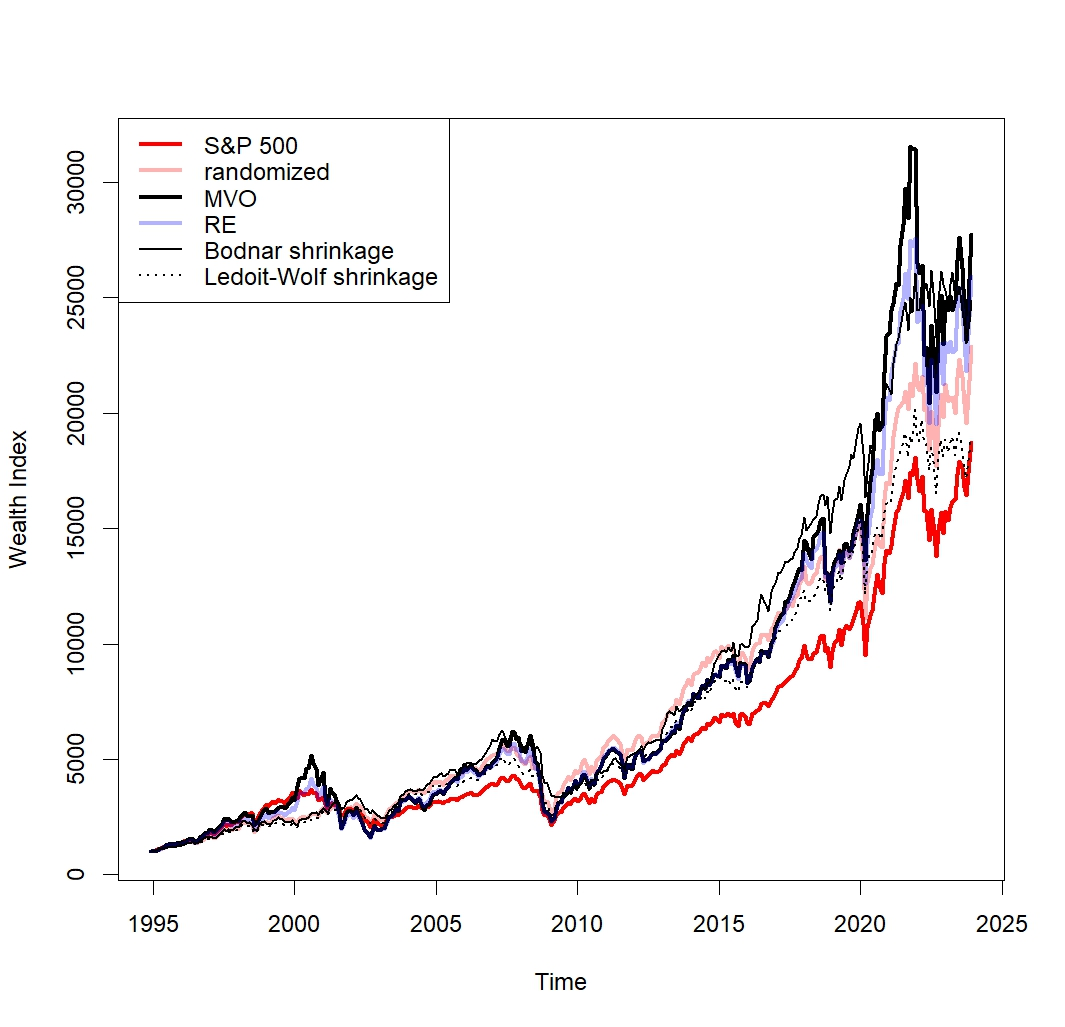
\includegraphics[width=.61\linewidth]{JPEGs/WealthIndex1.jpeg}
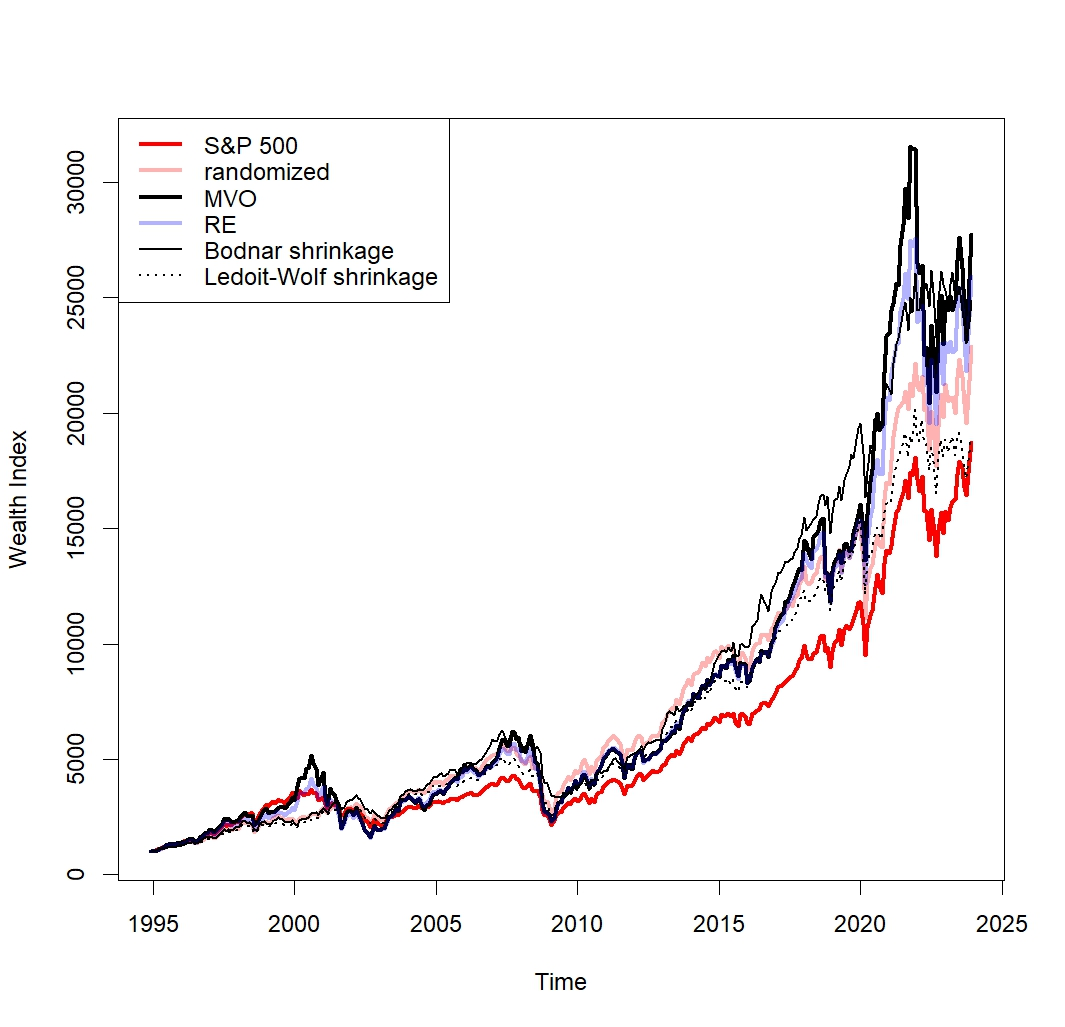
\includegraphics[width=.9\linewidth]{JPEGs/WealthIndex1.jpeg}
\caption{\label{fig:TotRetWeatlhIndexWithoutTranactionCosts}Growth of \$1000 by portfolio  per Total Return ignoring transaction costs, Jan 1995 - Dec 2023}
\end{figure}

\begin{figure}
\centering
%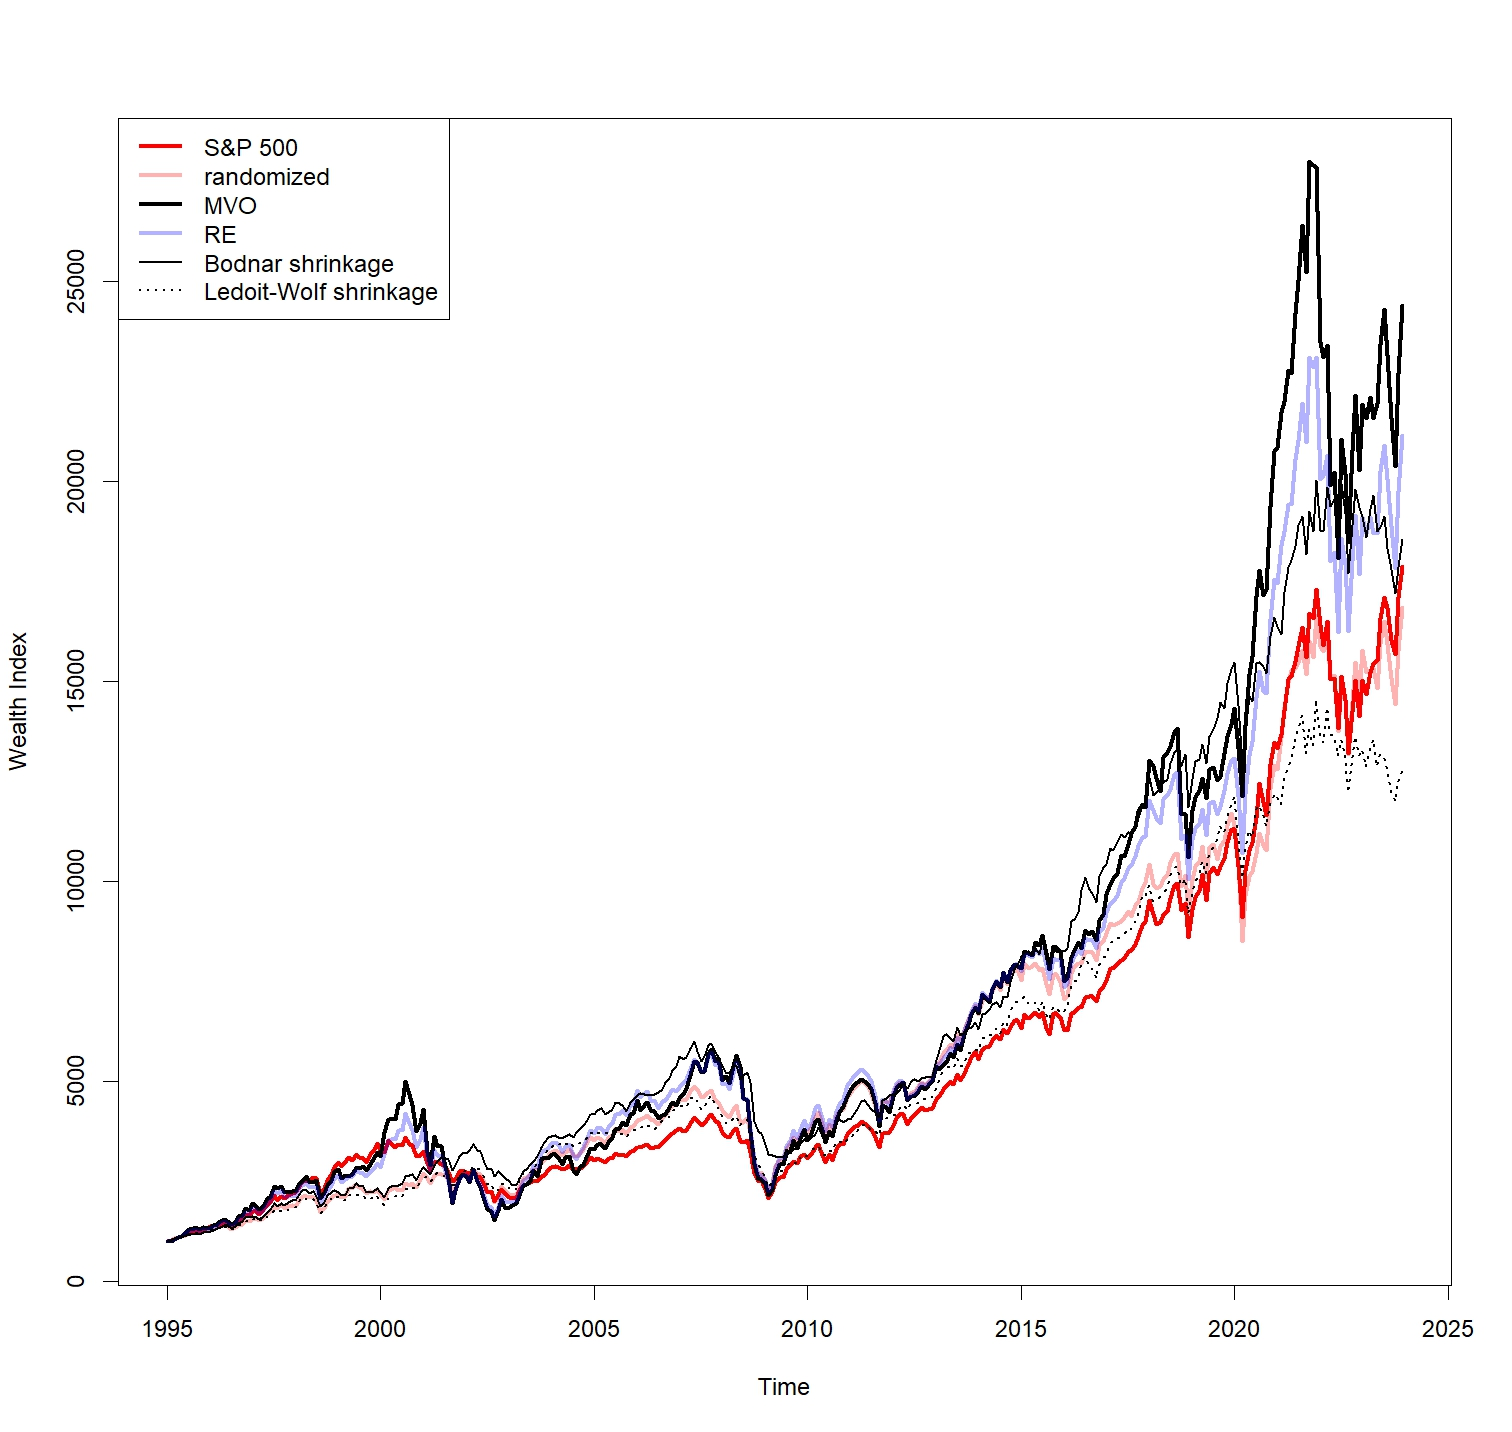
\includegraphics[width=.61\linewidth]{JPEGs/WealthIndex2.jpeg}
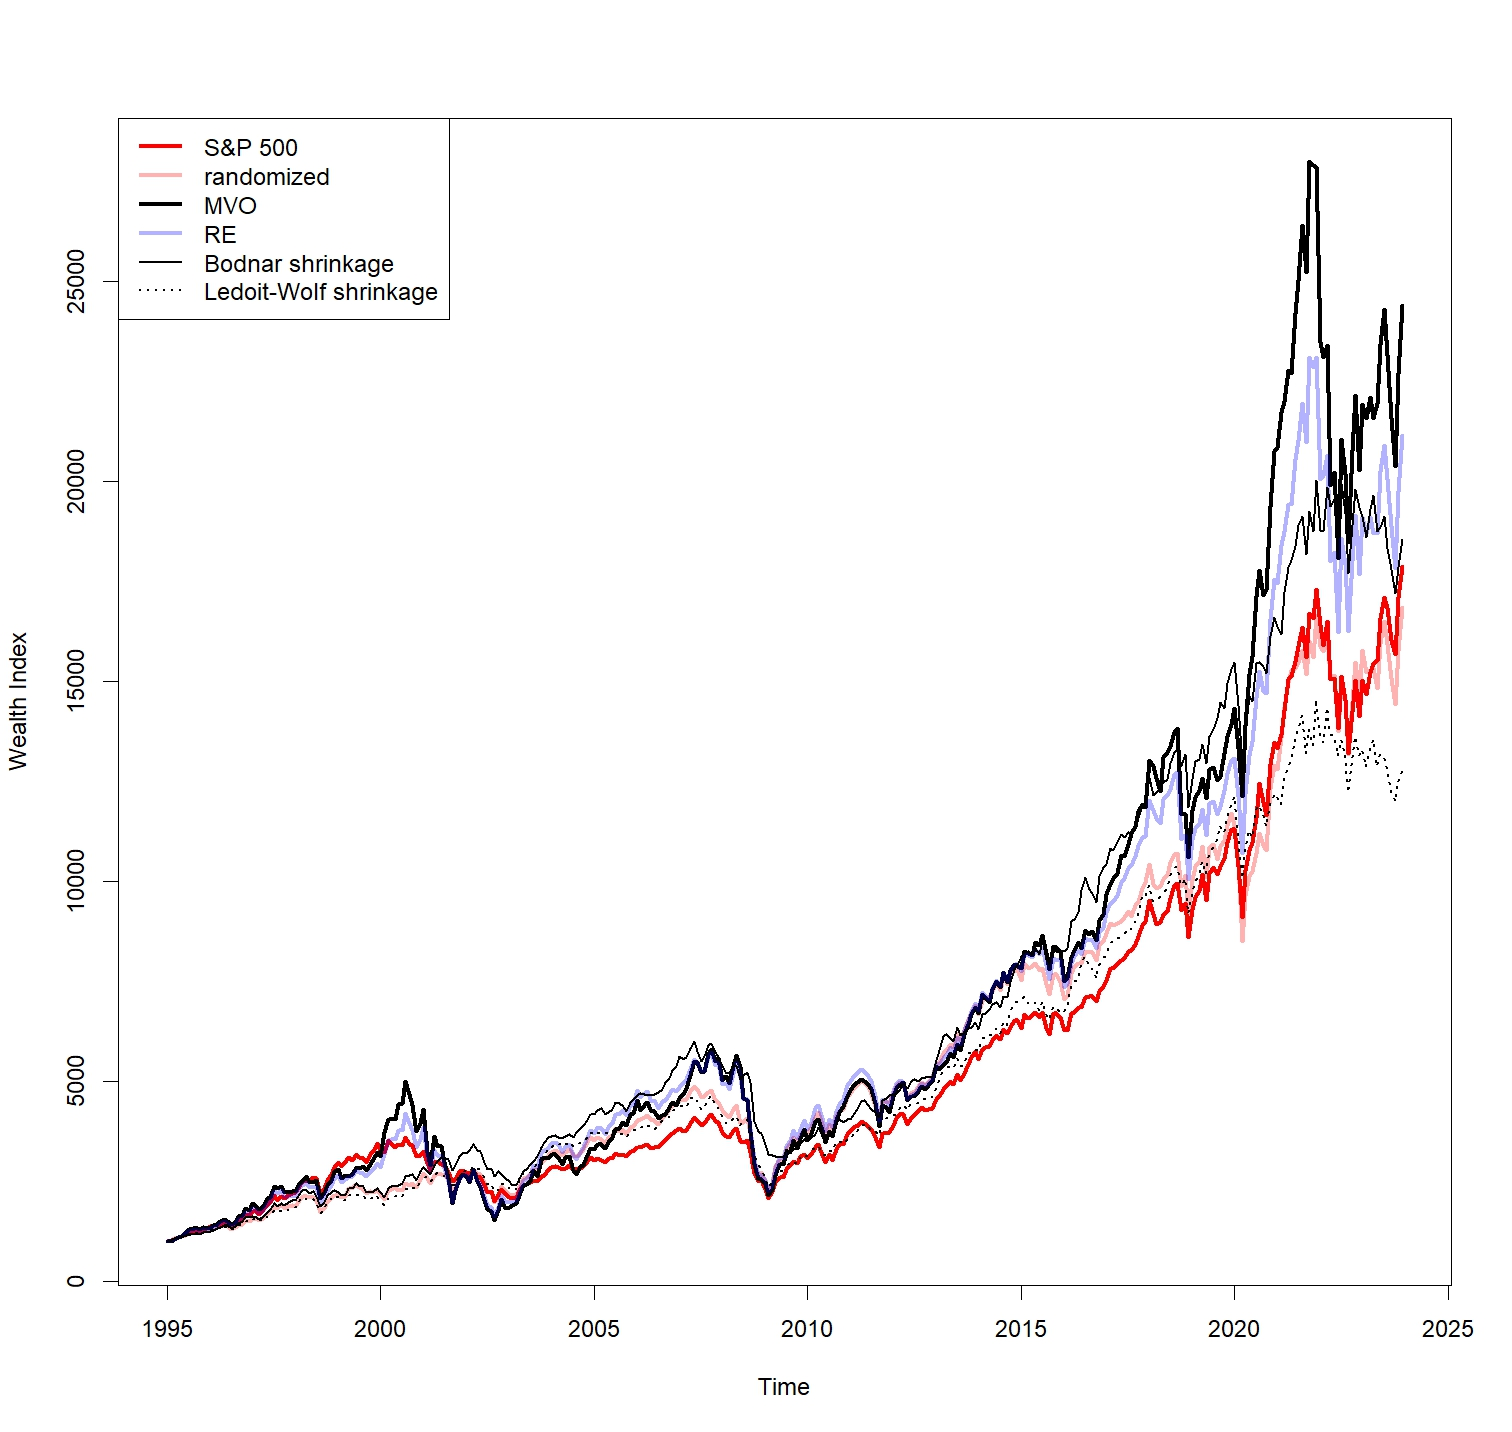
\includegraphics[width=.9\linewidth]{JPEGs/WealthIndex2.jpeg}
\caption{\label{fig:TotRetWeatlhIndexWithTransactionCosts}Growth of \$1000 by portfolio per Total Return with transaction costs, Jan 1995 - Dec 2023}
\end{figure}
\clearpage


\begin{figure}
\centering
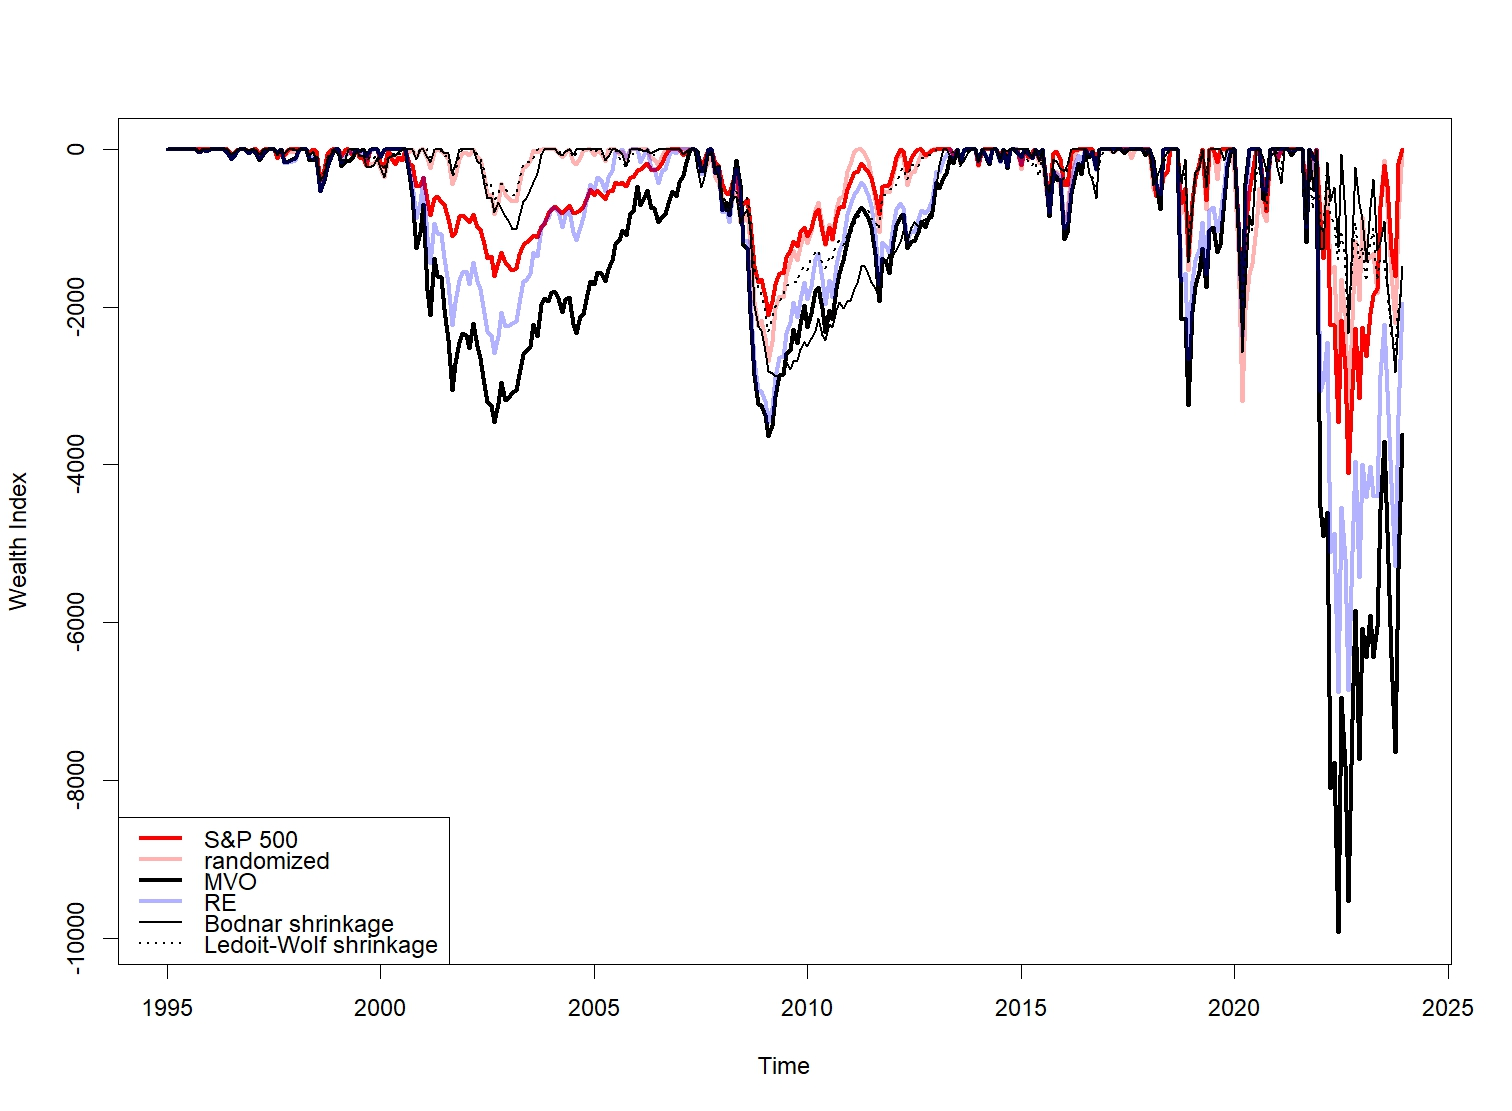
\includegraphics[width=.9\linewidth]{JPEGs/drawdowns.jpeg}
\caption{\label{fig:drawdowns}Drawdowns on \$1000 Wealth Index with transaction costs, Jan 1995 - Dec 2023.}
\end{figure}

\begin{figure}
\centering
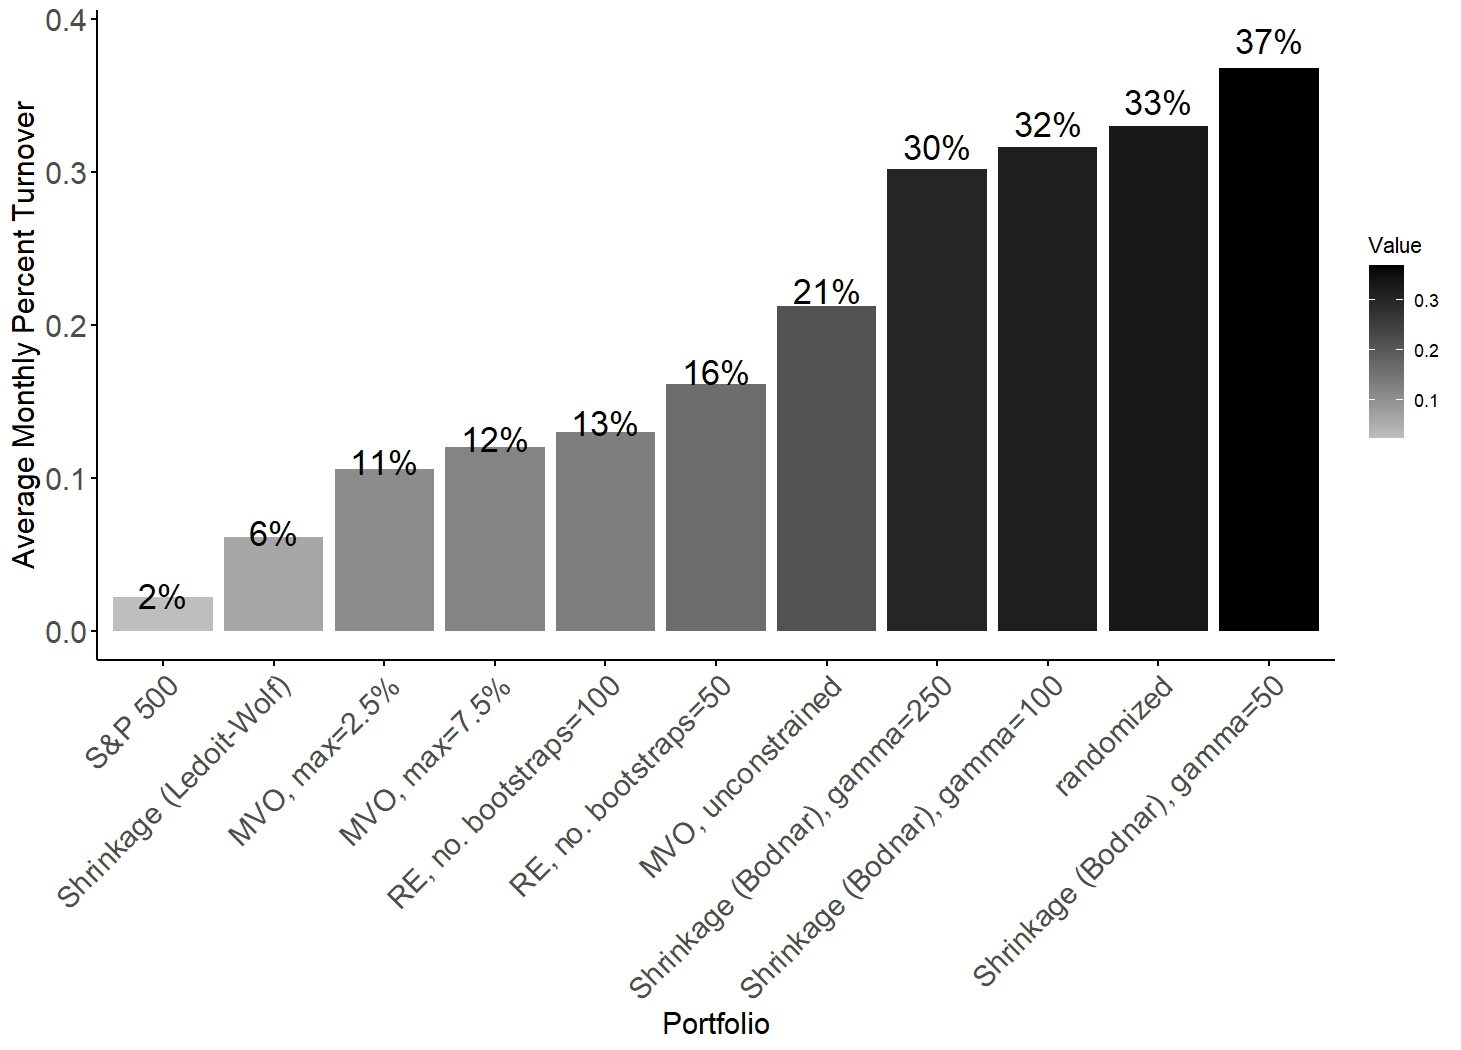
\includegraphics[width=.7\linewidth]{JPEGs/turnover.jpeg}
\caption{\label{fig:turnover}Average monthly portfolio Turnover due to Rebalancing, Jan 1995 - Dec 2023.}
\end{figure}
\clearpage

\begin{figure}
\centering
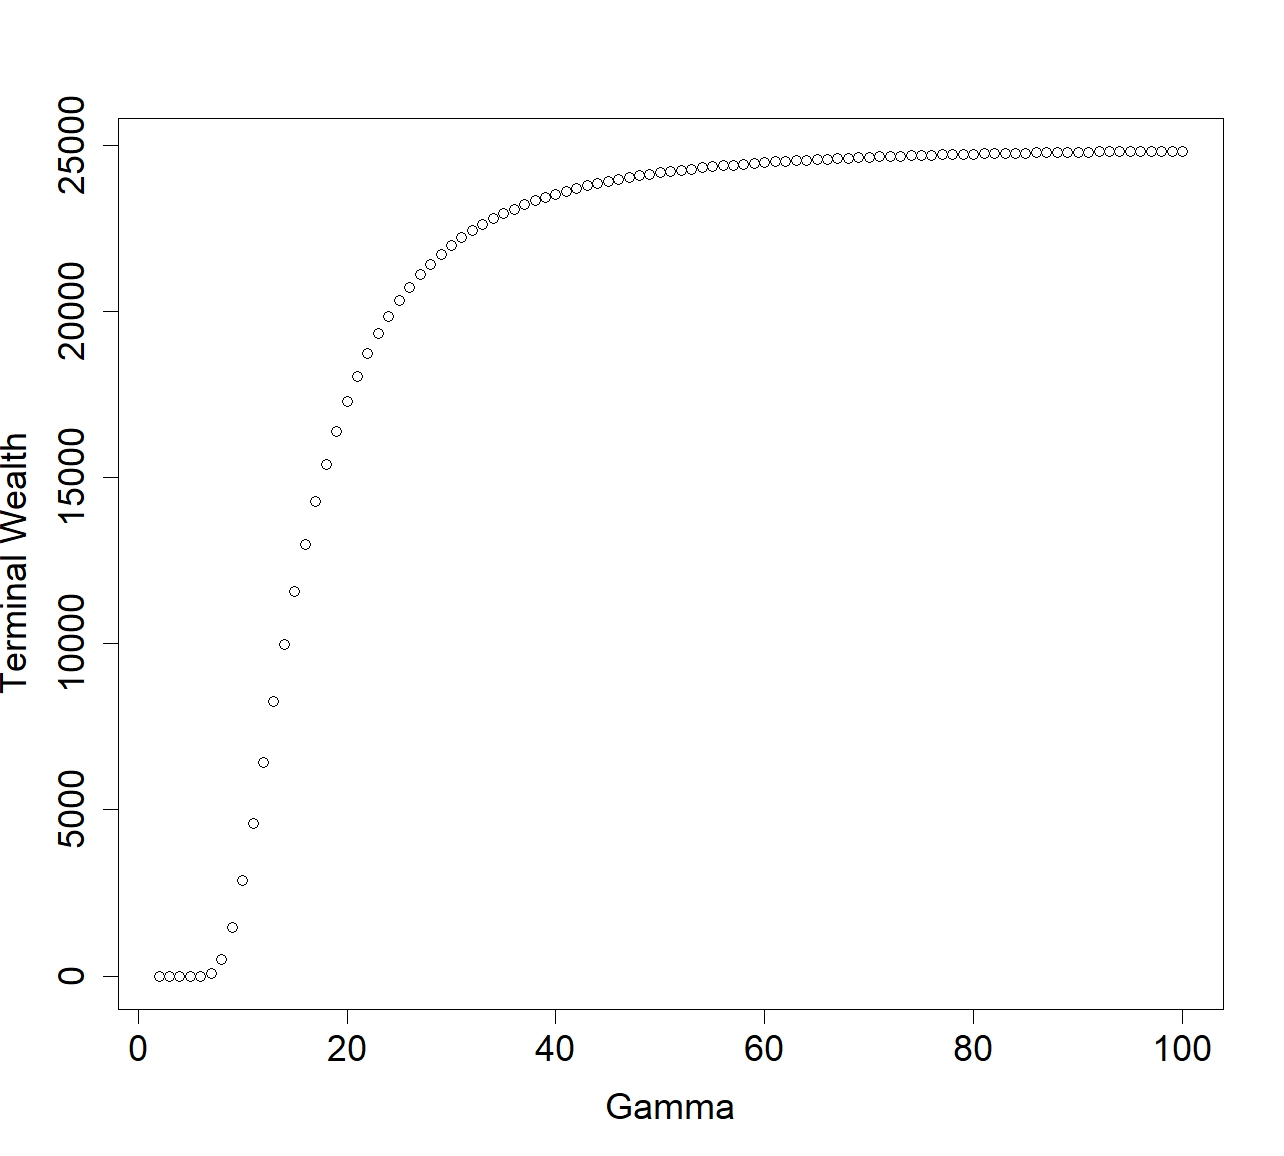
\includegraphics[width=.8\linewidth]{JPEGs/gamma_vs_Twealth.jpeg}
\caption{\label{fig:gamma_vs_Twealth}Bodnar Shrinkage Portfolios, gamma vs. terminal Wealth Index}
\end{figure}
\clearpage

\begin{figure}
\centering
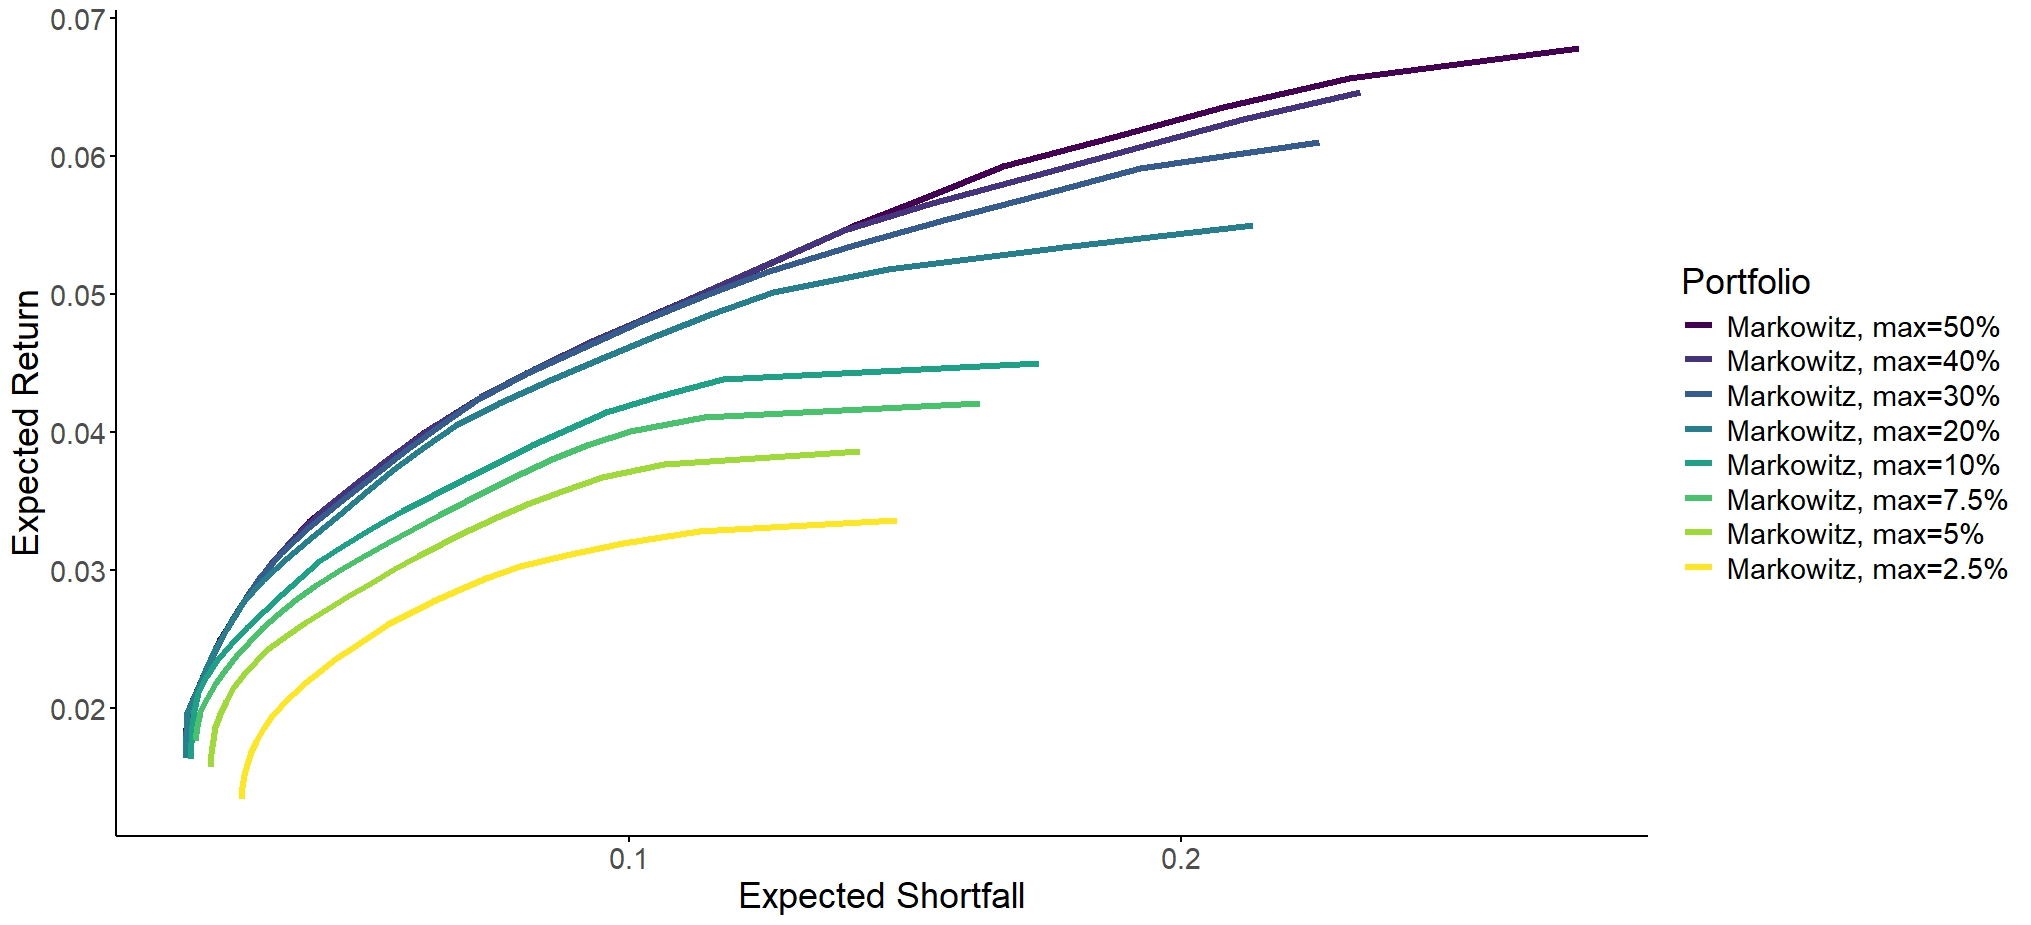
\includegraphics[width=1.05\linewidth]{JPEGs/EfficientFrontier.jpeg}
\caption{\label{fig:MarkowitzFrontiers}Efficient Frontiers of Constrained Markowitz Portfolios, Jan 1995 - Dec 2023.}
\end{figure}

\begin{figure}
\centering
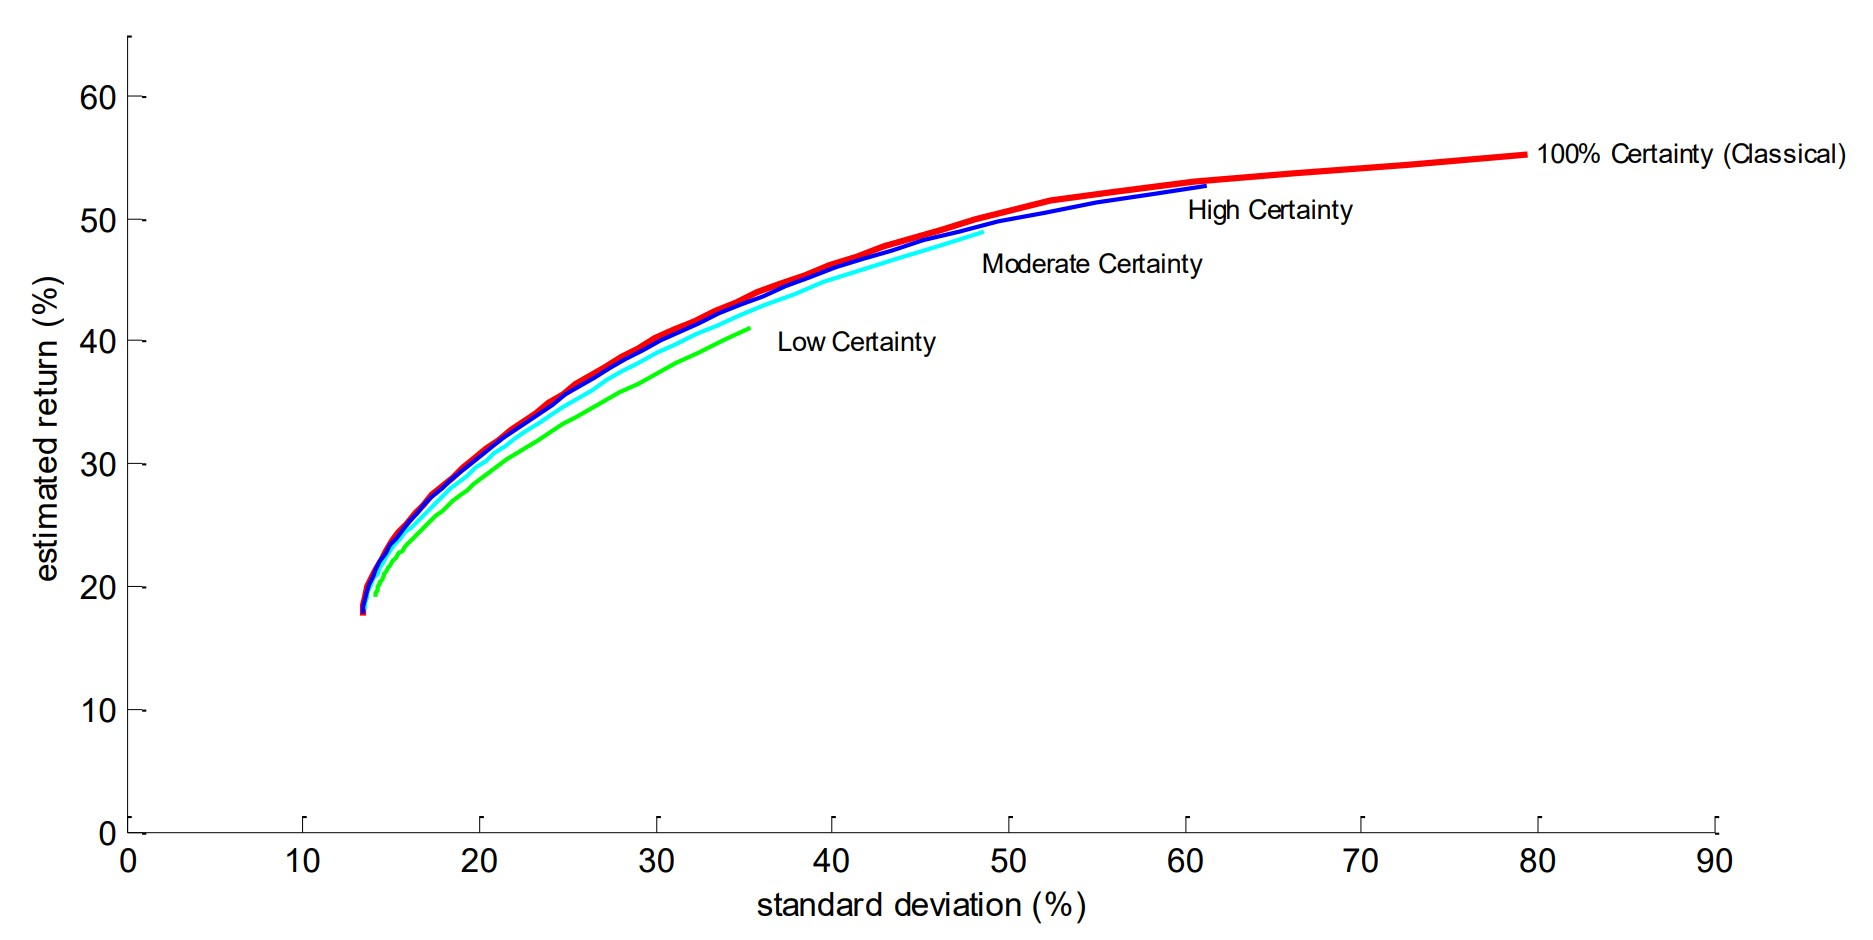
\includegraphics[width=1\linewidth]{JPEGs/MichaudFigure5.jpg}
\caption{\label{fig:MichaudFigure5} Figure 5 from Michaud and Michaud (2007).}
\end{figure}
\clearpage

\begin{figure}
\centering
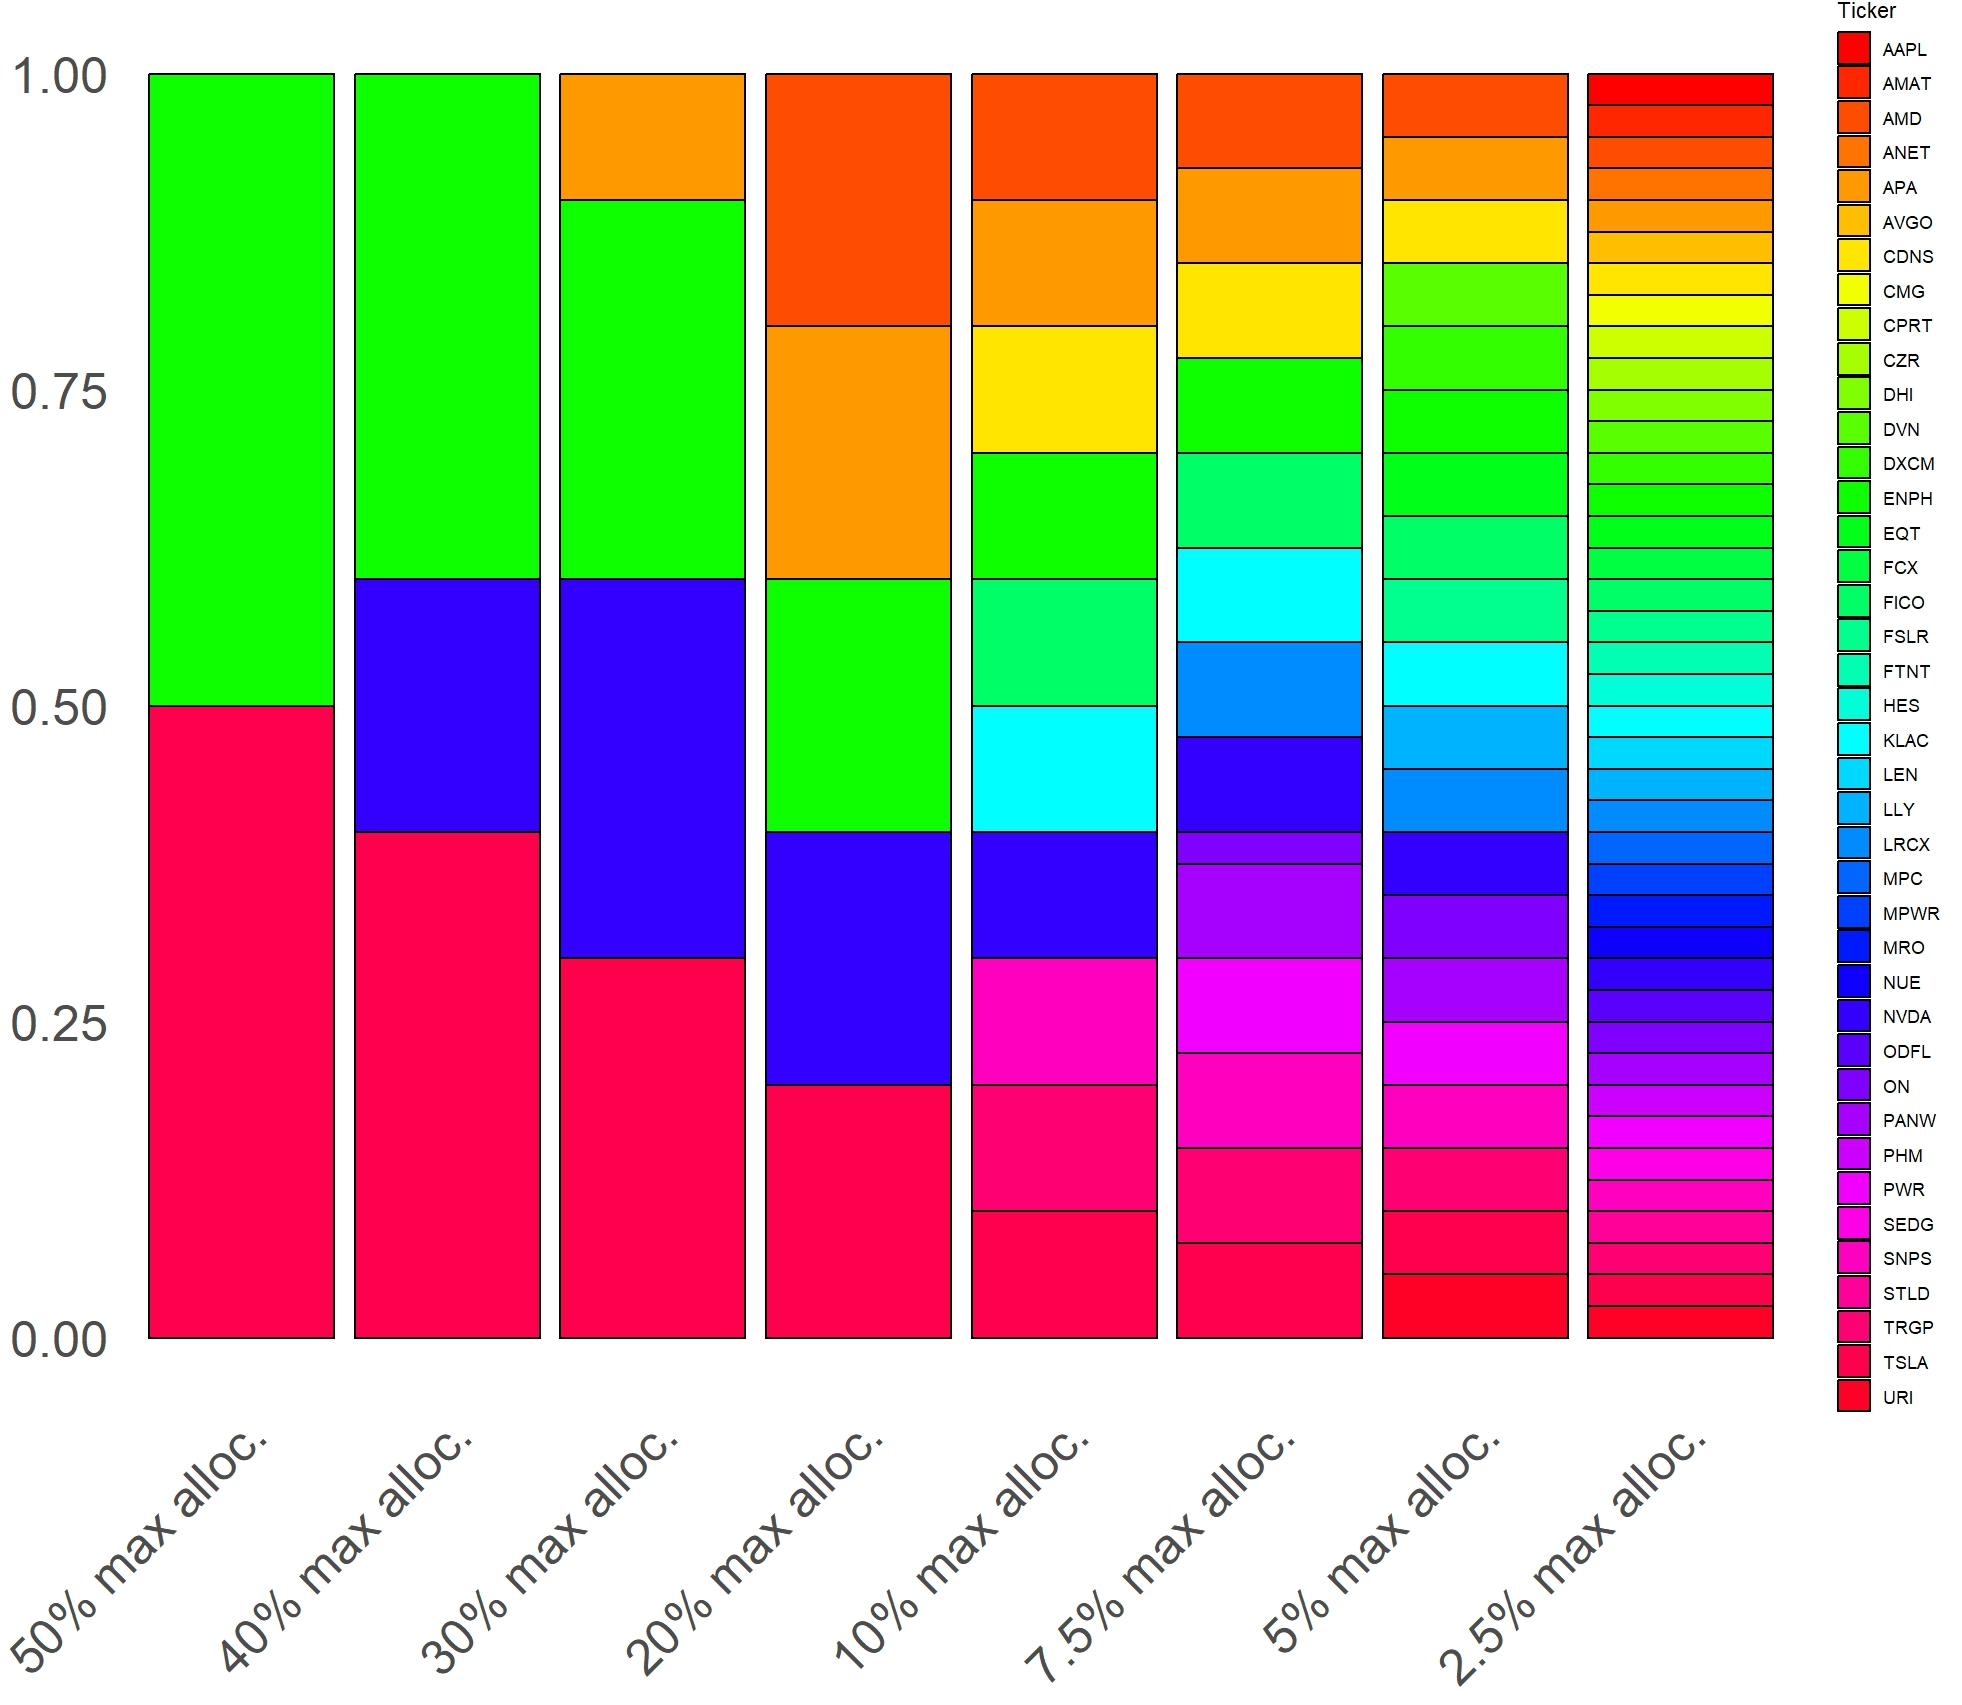
\includegraphics[width=1\linewidth]{JPEGs/MarkowitzCompositionMap.jpeg}
\caption{\label{fig:MarkowitzCompositionMap} Markowitz Portfolio Composition Map.}
\end{figure}
\clearpage

\begin{figure}
\centering
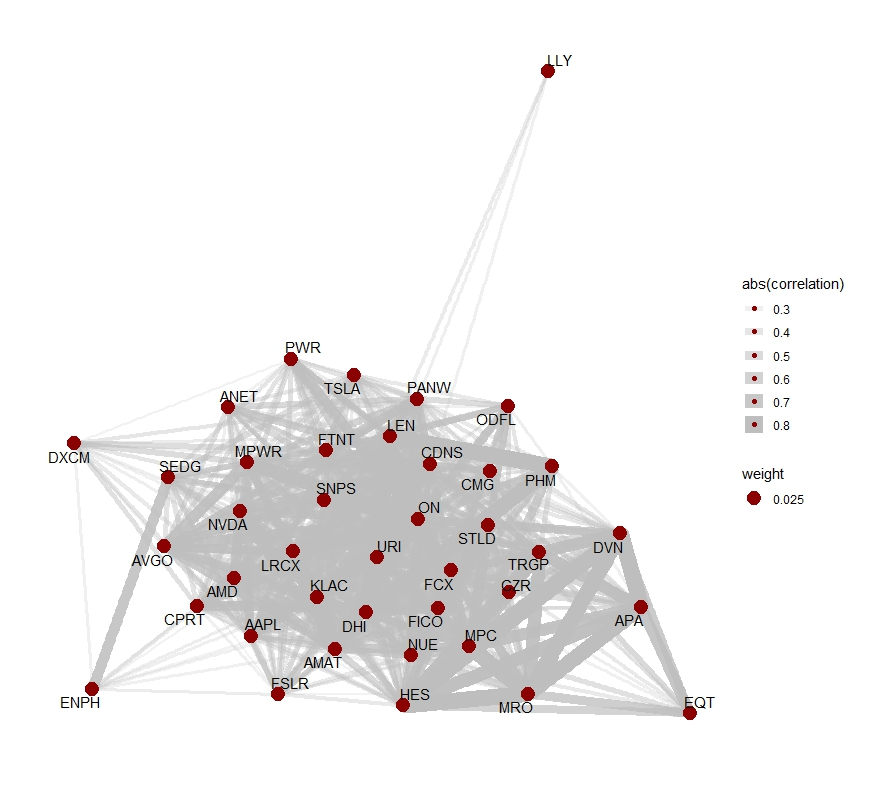
\includegraphics[width=1\linewidth]{JPEGs/MarkowitzCorrelationNetwork.jpeg}
\caption{\label{fig:MarkowitzCorrelationNetwork} Asset Correlation Network for a Markowitz portfolio with a 2.5\% maximum allocation constraint (rebalanced on Dec 2023).}
\end{figure}
\clearpage

\begin{figure}
\centering
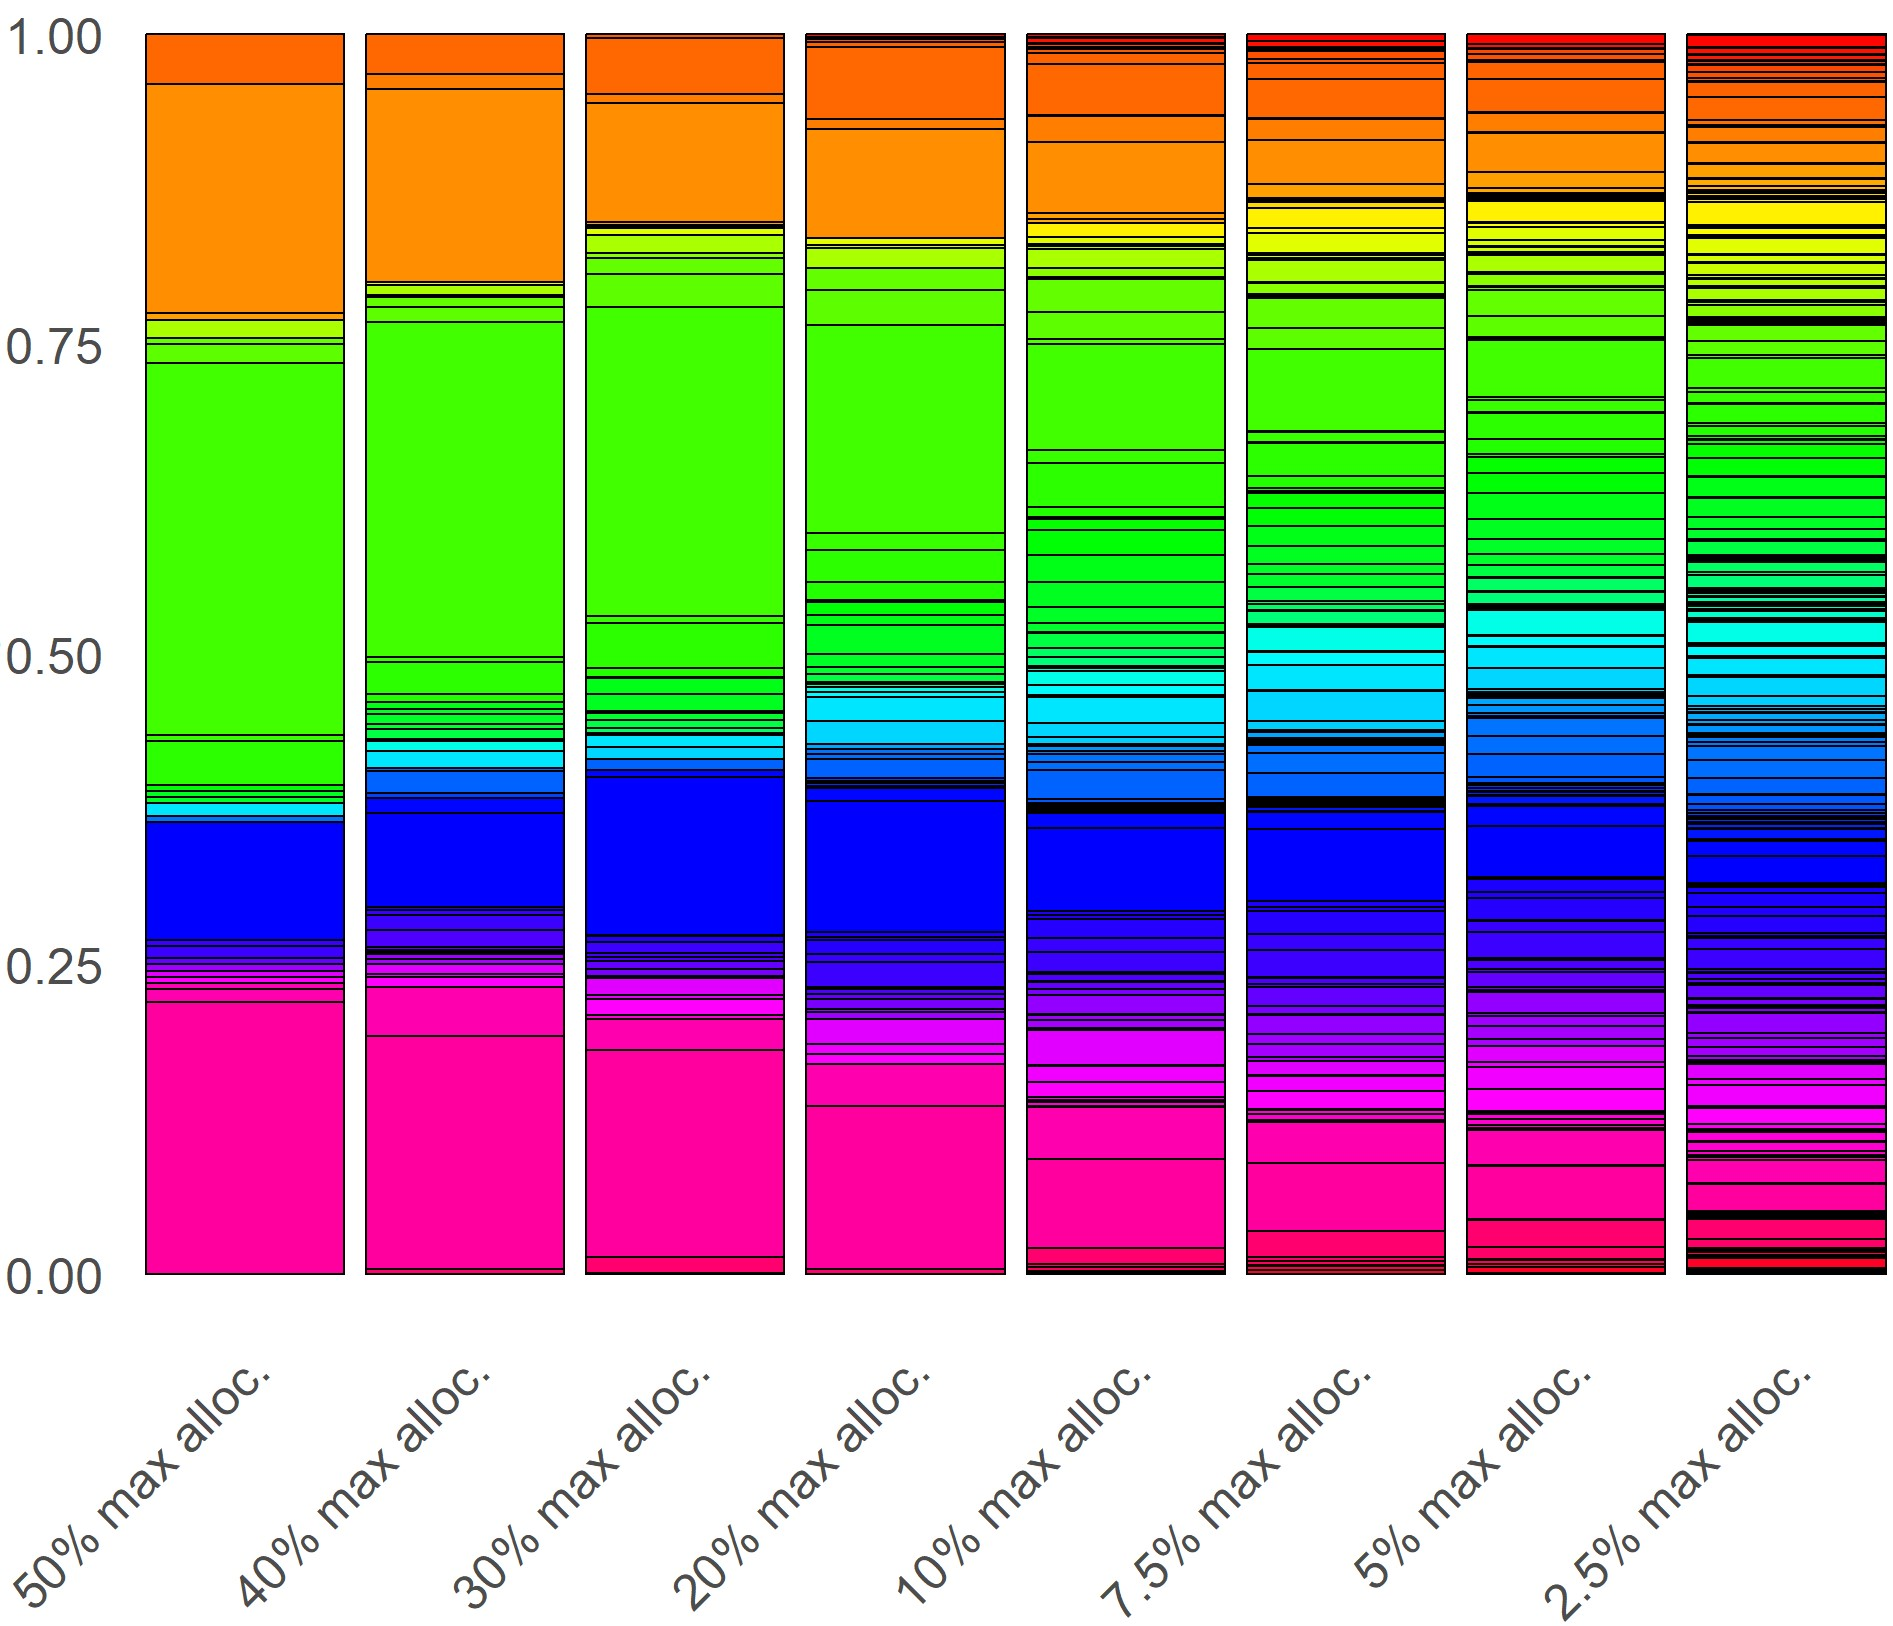
\includegraphics[width=1\linewidth]{JPEGs/MichaudCompositionMap.jpeg}
\caption{\label{fig:MichaudCompositionMap} Michaud and Michaud (2007) RE Portfolio Composition Map with 100 Monte Carlo simulations.}
\end{figure}
\clearpage

\begin{figure}
\centering
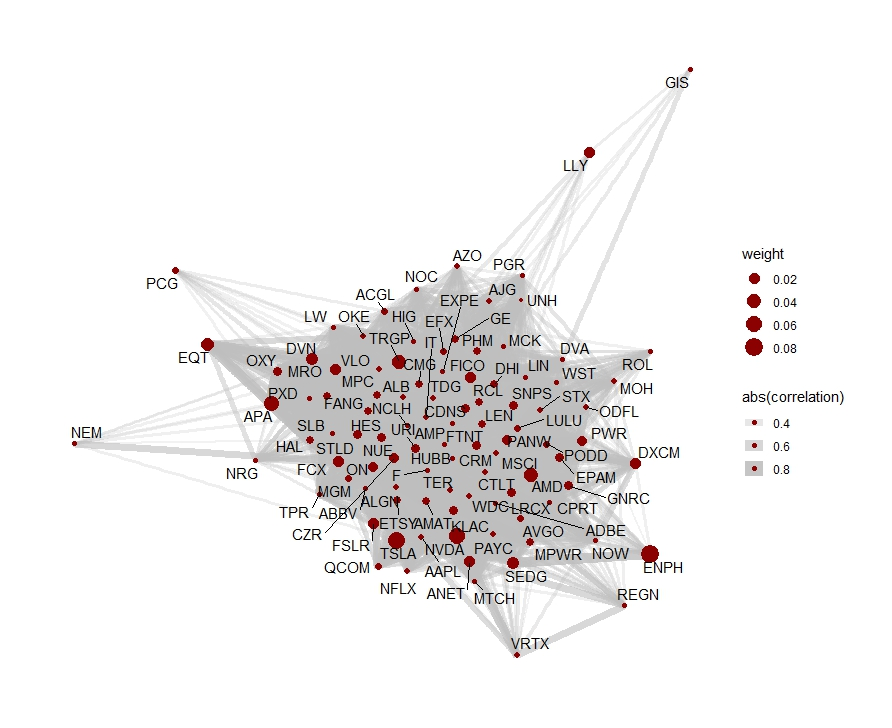
\includegraphics[width=1\linewidth]{JPEGs/MichaudCorrelationNetwork.jpeg}
\caption{\label{fig:MichaudCorrelationNetwork} Asset Correlation Network for an RE portfolio with 100 simulations and a 10\% maximum allocation constraint, (rebalanced on Dec 2023).}
\end{figure}
\clearpage

%\section{Appendix}

%\begin{figure}
%\centering
%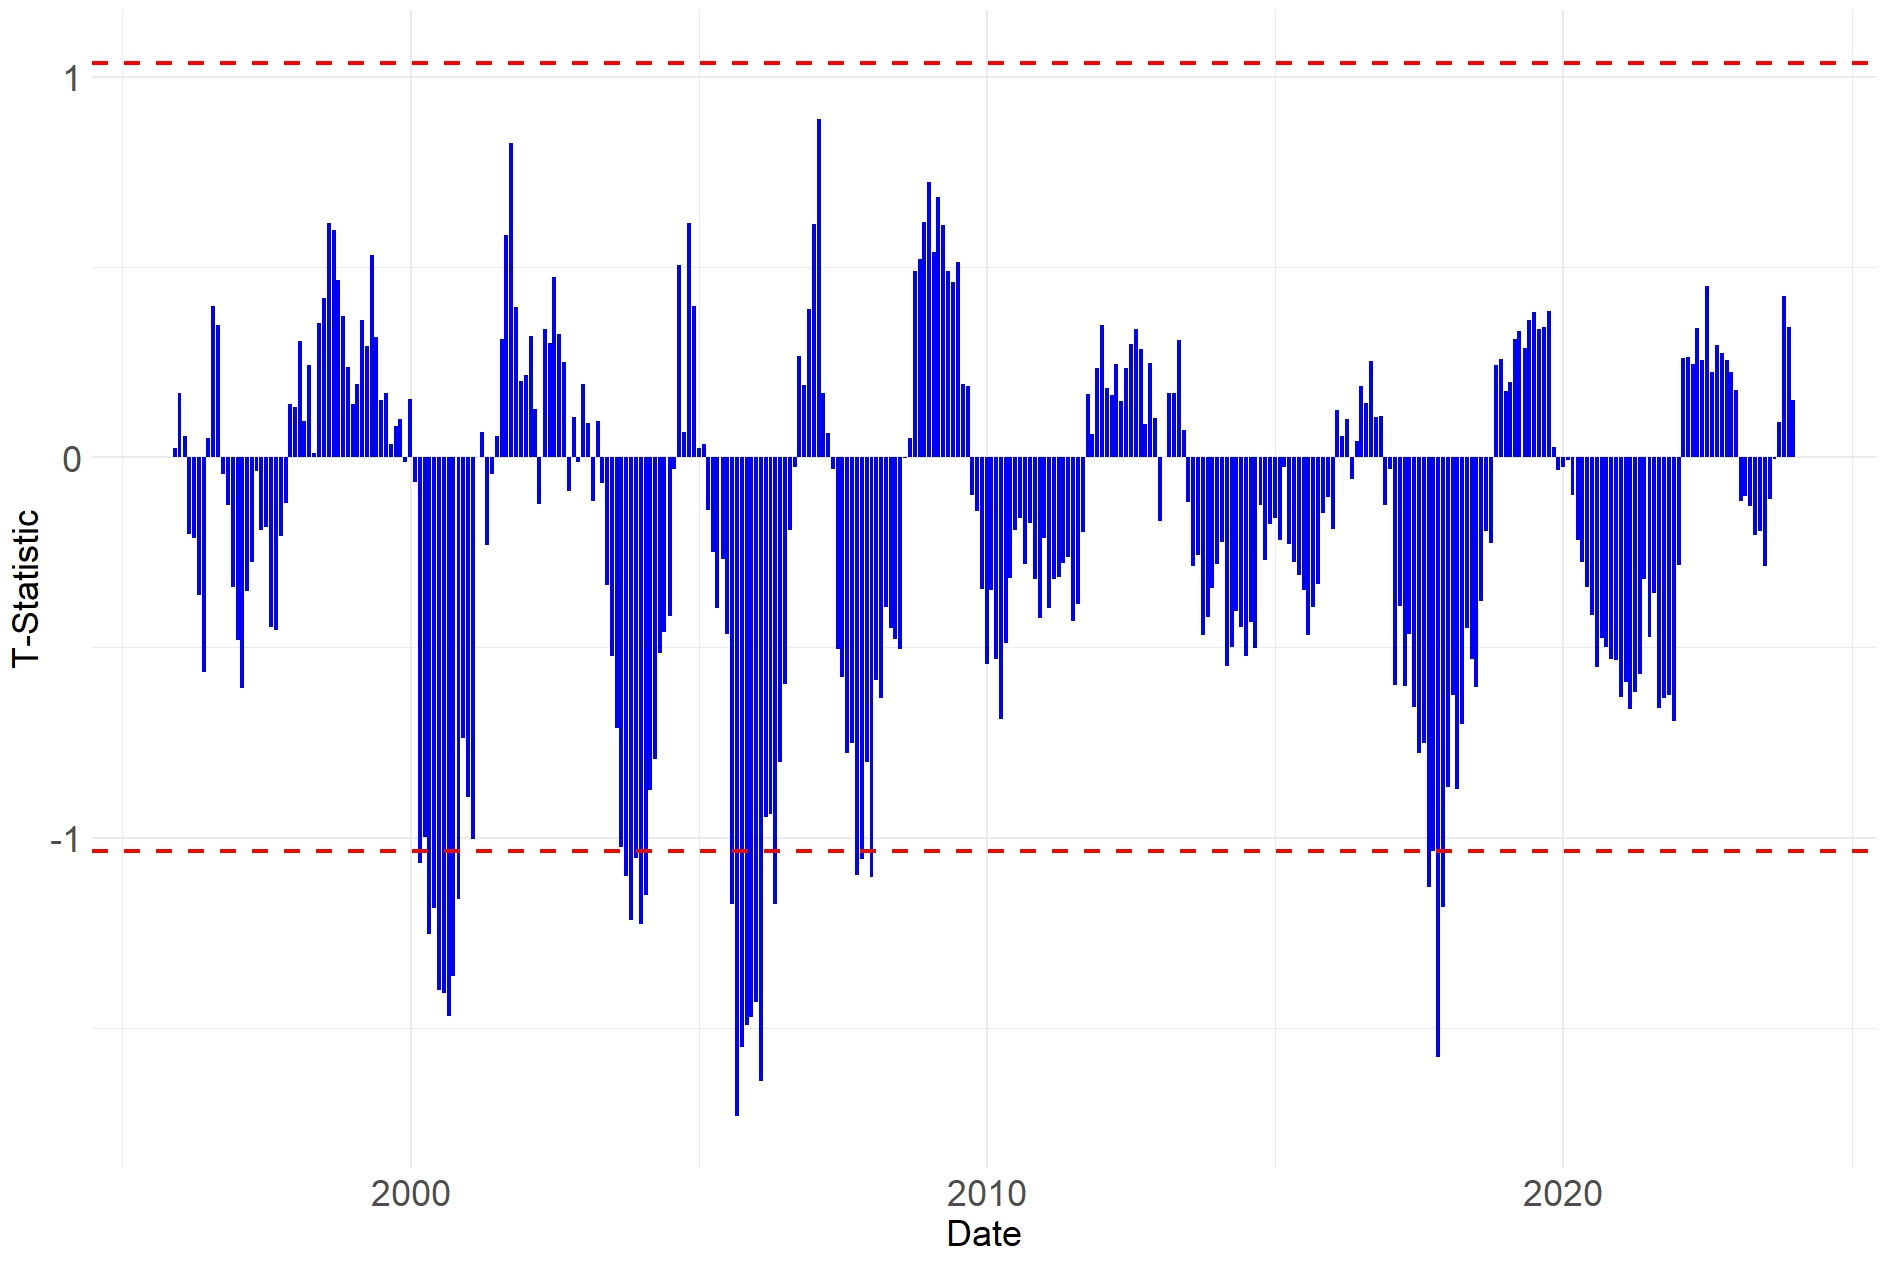
\includegraphics[width=1\linewidth]{JPEGs/tStat_chart.jpeg}
%\caption{\label{tStat_chart} 12-month rolling T-Test with a 70\% Confidendce Interval, Markowitz Portfolio with a 2.5\% maximum allocation constraint vs. cap-weighted S\&P 500 total returns.}
%\end{figure}
%\clearpage

\end{document}